\documentclass[11pt]{article}
\usepackage{adjustbox}
\usepackage{lipsum}% example text
\usepackage{chngpage}
\usepackage{graphics}
\usepackage{float}
\usepackage{multicol}
% \usepackage{amsmath}
\usepackage[font=scriptsize]{caption}
\documentclass[11pt]{article}
\author{HCEL}
\date{TBD} 
\title{TBD}


\usepackage{authblk}
\usepackage[utf8]{inputenc}
\usepackage{graphicx}
\usepackage{amsmath}
\usepackage[margin=1in]{geometry}
%\usepackage[latin1]{inputenc}
\usepackage[english]{babel}
\usepackage{natbib}
\usepackage{amsmath,amsfonts,amssymb,amsthm}
\usepackage{dsfont}
\usepackage[official]{eurosym}
\usepackage{graphicx,graphics}
\usepackage{booktabs}
\usepackage[flushleft]{threeparttable}
\usepackage{url}
\usepackage[breaklinks=true]{hyperref}
\usepackage{pdflscape,pdfpages}
\usepackage{xcolor,colortbl}
\usepackage{rotating}
\usepackage[justification=justified]{caption}
\usepackage{subcaption}
\usepackage{subfiles}
\usepackage[toc, page]{appendix}
\usepackage{comment}
\usepackage{bbm}
\usepackage{float}
\usepackage{pict2e}
\usepackage{tikz}
\usetikzlibrary{patterns}
\usepackage{geometry}
\newcommand*{\BibPath}{}
\bibliographystyle{chicago}
\definecolor{dark-red}{rgb}{0.4,0.15,0.15}
\definecolor{dark-blue}{rgb}{0.15,0.15,0.4}
\definecolor{medium-blue}{rgb}{0,0,0.5}
\hypersetup{
 colorlinks, linkcolor={dark-red},
citecolor={dark-red}, urlcolor={dark-red}
}
\usepackage{mdframed}
\mdfdefinestyle{MyFrame}{%
    linecolor=black,
    outerlinewidth=2pt,
    %roundcorner=20pt,
    innertopmargin=4pt,
    innerbottommargin=4pt,
    innerrightmargin=4pt,
    innerleftmargin=4pt,
        leftmargin = 4pt,
        rightmargin = 4pt
    %backgroundcolor=gray!50!white}
        }
%\usepackage{aer}
%\usepackage{endfloat}  
%\graphicspath{{figures/}{../figures/}}
\hypersetup{colorlinks,linkcolor={blue!50!black},citecolor={blue!50!black},urlcolor={blue!80!black}
}
%\linespread{1.3} %1.2
\usepackage{setspace} % Avoiding \linespread because it then applies to footnotes as well.
\onehalfspacing
\setlength{\bibsep}{0.1pt plus 0.5ex}
\setlength{\parindent}{0pt} %indentation space: here no indentation
\setlength{\footnotesep}{0.3cm} %vertical space between footnotes
\setlength{\bibhang}{1em}

\usepackage[capitalize]{cleveref}
\begin{document}
\title{\textbf{Boxed Opportunities: The Effects of Amazon \\ Fulfillment Centers on Regional Employment \\ and Income Mobility }}
\author{Harvard College  Economics Labs \and Shivant Krishnan (Project Lead)* \and Brayant De Leon, Nicolas Marin Gamboa, Ian Magnell,  Timothee Maret (Analysts)\footnote{The authors are from The University of Chicago. We are grateful to Gregory Wright, Ian Seyal, and the Brookings Institution for invaluable feedback and advisory. We also thank Professors John List, Michael Kremer, and Min Sok Lee for their supportive contributions.}}
\date{Spring 2023}
\begin{figure}[t]
\centering

\includegraphics[width=5cm]{Eclabs_logo.png}
\end{figure}

\maketitle
\newpage
\tableofcontents
\newpage

\section{Team and Project Overview}
\subsection{Harvard College Economics Labs}

\-\hspace{0.5cm} Harvard College Economics Labs is a group of undergraduate researchers at Harvard, UChicago, and Stanford that completes pro-bono economics research for governments, think tanks, and other social enterprises. The organization is advised by Harvard graduate researchers and faculty members. Its past and current research partners include the United Nations Development Programme (UNDP), the Virginia Department of Education, the climate think tank E3G, and the Environmental Protection Agency (EPA). More information can be found on \hyperlink{www.harvardeconomics.org}{our website}.

\subsection{Project Partner: Brookings Institution}

\-\hspace{0.5cm} The Workforce of the Future initiative at Brookings produces research to diagnose and counter trends relating to the availability of middle-class jobs and the decline in upward mobility for millions of workers. At the core of the initiative is a body of research that uncovers local economic growth strategies to create high-wage jobs in fast-growing sectors of the economy. The research—most recently described in the initiative’s 2021 report, “Moving Up," puts a spotlight on who is falling behind, where, and by how much. It also identifies career pathways that should be expanded to improve economic opportunity for those being left behind. This research informs the initiative’s Smart Growth Cities tool, an online tool that helps local economic development officials choose a successful growth strategy and provides a detailed analysis of the workforce implications of that strategy.

\subsection{Project Overview}

\-\hspace{0.5cm} The objective of this project is to assess the impact of Amazon Fulfillment Centers in two dimensions: the employment effects and labor shortages produced by warehouse employment opportunities; and the long-term mobility potential for the individual worker. We construct two models with regional employment and post-transition income change as our variables of interest. Further, we suggest policy implications to address these complex challenges, hoping that our findings offer a new approach to better understand the contours of intragenerational mobility and unemployment. 

\clearpage

\section{Results in Brief}

\-\hspace{0.5cm} In our analysis, we investigate these two implications of warehouse employment using descriptive economic models, particularly difference-in-difference and fixed-effects regression. Overall, we observe a significant warehouse-induced impact on the rate of warehouse employment in a given county and the proportion of warehouse jobs that are taken up. However, we do not find a significant impact of Amazon Fulfillment Centers on total county employment, potentially due to the movement of workers from local industries to warehouses. In addition, we do not find clear evidence that such job opportunities are associated with increased income during the years following a person's Amazon employment. Our results broadly suggest that the industry wage models may be unrepresentative of the average blue-collar warehouse worker and his mobility potential.

\section{Background}
\-\hspace{0.5cm} Amazon is more than just another large corporation; since its founding in 1994, the online retail giant has expanded to over 175 Fulfillment Centers where incoming orders are received, packed, and shipped out to its 310 million customers. In order to achieve such an expansive distribution network Amazon has received millions in tax credits, exemptions, and infrastructure assistance from state and local governments across the US with the objective function of  economic prosperity. Warehouse jobs tend to be particularly enticing to low-income populations that contain job-hungry workers in search of better prospects, but this comes at a significant cost. In particular, when policymakers discuss the mobility potential of warehouse/logistics sector jobs, they often lump together blue-collar roles with managerial and other high-wage positions. 

\-\hspace{0.5cm} An analysis of these claims is timely. Despite the success and influence of Amazon, localities face increasing competition for the establishment of Amazon Warehouses. Further, Amazon reports creating hundreds of thousands of jobs with competitive pay and benefits, but some concerns arise regarding recent worker sentiment reports. A prominent lack of job satisfaction has been identified in annual reports and qualitative interviews of Amazon's lower-wage employees -- According to the US Department of Labor, this is attributable to the long working hours and physically injurious tasks with which those employees are faced. 

\-\hspace{0.5cm} Broadly, we hope to disaggregate the various roles within Amazon warehouses and suggest that the industry wage models are not reflective of the average warehouse worker. This body of research suggests that Amazon Fulfillment Centers may restrict the future socioeconomic benefits that a worker, particularly a low-income one, can derive from their labor. Studying the employment and mobility effects of Amazon Fulfillment Center openings is thus a keen opportunity for us to harness empirical tools and weigh in on this debate. In the present study, we use publicly available data on US county and sector employment, and panel occupational data for individual Amazon workers, to undertake a rigorous economic evaluation of Amazon's job growth and income mobility claims.
\clearpage 

\section{The Literature}
\begin{text}

\begin{center}
    \textbf{Prior Research on Employment}
\end{center} 

\-\hspace{0.5cm} The warehousing industry is a crucial component of the global economy, serving as an intermediary for the movement of goods between manufacturers and consumers. The Bureau of Labor Statistics cites that employment in the warehousing industry has grown significantly over the past decade, from 700,000+ workers in 2013 to 1.93 million workers in 2023, recently offering an average hourly wage of around \$23.25. The rise of e-commerce and the increasing demand for more efficient delivery of goods has led to significant changes in the warehouse industry. Similarly, the COVID-19 pandemic placed several additional constraints on warehouses, including: social distancing; space and capacity issues; and reshoring manufacturing due to global supply chain shocks. Despite the changing landscape of this industry, warehouse employers continue to promise vast benefits of this employment on both group and individual levels. Literature suggests that the warehouse industry is riddled with hardship due to difficult manual labor and its deceptive treatment of employees -- so perhaps, it does not fulfill its intended promises.

\-\hspace{0.5cm} Additionally, the warehouse industry is heavily reliant on the use of temporary agency workers (Rydstorm et al. 2023). This characteristic arises due to the widely used ‘just-in-time’ production/delivery approach.  This strategy is motivated by the benefits of a highly flexible workforce and, thus, its ability to maintain efficient supply chains while mitigating unnecessary costs. A survey conducted in Illinois suggested that 63\% of workers in the warehouse industry were temporary workers, with a median pay of \$9.00 per hour, \$3.48 less than direct hires (Warehouse Workers for Justice). The use of temporary agency workers is likely to persist over the next decade as warehouses are reluctant to experiment with emerging technologies, which, in time, may also disrupt the industry. For example, the adoption of artificial intelligence and automation can displace many warehouse workers, leaving them with limited options for short-term employment (Gutelius 2021). We note that the employment of temporary workers, warehouse management, and operations, is typically outsourced to third-party logistic firms, which further differentiates temporary workers from direct hires. More importantly, the presence of inequality, associated with race/ethnicity, immigration status, and gender, between warehouse workers is an ever-growing concern. Research substantiates the fact that immigrant women, Latina women, and women of color are often the most subordinated workers.  Together, these differences lead to lower wages, lower positions, and unpromising future employment mobility.

\-\hspace{0.5cm} A 2011 study especially informs our approach in examining the labor market effects of Amazon Fulfillment Centers. The authors employ a comprehensive dataset of historical employment statistics in West Germany between 1994 and 2002 to examine the impact of new firm creation on job growth in different industries and regions. They find that newly established businesses play a significant role in generating increases in employment, but with varying effects depending on the industry and regional characteristics (Fritsch \& Schindele, 2011). The study highlights that factors such as the size and age of businesses, as well as the industrial structure of certain regions, can influence the employment contributions of new firms.  

\-\hspace{0.5cm} Although Fritsch \& Schindele explore these questions in an entirely different context than the present study, their framework has been incredibly valuable in ideating and executing our analyses. Specifically, we see that the employment effects of Amazon Warehouses can be teased out by considering factors such as the number of warehouses, the size of the workforce, and the regions in which they operate. This informs our use of employment-to-population ratio as an outcome variable, as well as county-by-county analysis with fixed effects to estimate treatment heterogeneity. Their study utilizes a cross-comparison of different industries, such as service and manufacturing, which inspires our comparison between the warehouse industry and other employment sectors. These comparisons allow us to identify the particular effects of the introduction of new Amazon Warehouses across the US, and more broadly, to assess Amazon's implications for regional employment trends and job growth. As follows, these conclusions aim to inform the development of policy which addresses the macro- and micro-challenges associated with warehouse employment and its characteristic hindrance of long-term mobility potential for individual workers.\bigskip

\begin{center}
    \textbf{Prior Research on Mobility}
\end{center} 

\-\hspace{0.5cm} Economic mobility refers to the ability for an economic agent, i.e. an individual or family unit, to improve their economic status over time. This phenomenon can be measured across generations (inter-generational mobility) or within the same generation (intra-generational mobility), noting that the present study emphasizes the latter. Economic mobility is a crucial area of study since it reveals the barriers faced by some individuals in obtaining better long-term socioeconomic outcomes. Further, this field informs public policy relating to improving equality of opportunity and reducing income inequality. In this section, we provide an overview of the existing literature on mobility, defining a few key theories and contextualizing them within past/current empirical studies. We then address two articles that were particularly useful in the development of this study, in which the authors analyze earnings inequality and long-term mobility potential of people employed in the warehousing industry.

\-\hspace{0.5cm} Becker \& Tomes (1979) present the seminal model of inter-generational income transmission, suggesting that parental investments in human capital are a key determinant of their children's income as adults. Assuming that each family intertemporally maximizes a utility function,  the preference relation not only depends on the consumption of the parents but also the quantity and quality of their children. When families increase investment into human and non-human capital, the incomes of their children increase. This article suggests that the family's "endowment" of genetically determined race, ability, and other characteristics mediates the link between parent investment and child fortunes. 

\-\hspace{0.5cm} Similarly, Chetty et al. (2014) conduct several influential empirical studies on US economic mobility. They find that there exists significant regional variation in income mobility potential, and importantly, that on average, a 10 percentile increase in parent income is associated with a 3.4 percentile increase in a child’s income. Further geographic analysis confirms that high-mobility areas exhibit several characteristics, including:
\begin{enumerate}
    \item Less residential segregation
    \item Less income inequality (measured by Gini coefficient)
    \item Higher primary school quality
    \item Greater social capital
    \item Greater average family stability.
\end{enumerate} 
\-\hspace{0.5cm} To this end, Chetty et al. develop the first publicly available descriptive statistics on US intergenerational mobility, which pave the way for a vast body of research in this regard. While the above theoretical and empirical frameworks are not directly adopted by the present study, they provide critical intuition regarding the roles of family structure, educational quality, and other subtle determinants of economic mobility. More precisely, they provide insight into the regional heterogeneity of mobility trends, which are consistently addressed in our analysis of Amazon Fulfillment Centers. 

\-\hspace{0.5cm} We finally address two recent mobility studies that are particularly relevant to the present research. The first is a case study of California's Inland Empire entitled “Warehouse Employment as a Driver of Inequality in the Inland Empire: The Experiences of Young Amazon Warehouse Workers.'' Here, the authors investigate the relationship between temporary employment and earnings inequality in the context of Amazon warehouse work. The study also includes a series of in-depth qualitative interviews of Amazon employees which may suggest that there is a mismatch between expectations and reality for this type of employment. The authors suggest that the rise of temporary employment in this industry has exacerbated wage disparities and created exploitative working conditions (Reese \& Scott, 2019). They specifically focus on the role of staffing agencies in perpetuating this inequality, as these agencies often provide job-hungry workers -- such as those in the Inland Empire region -- with unstable and low-wage jobs. Another study by De Lara (2013) entitled “Warehouse Work: Path to the Middle Class or Road to Economic Insecurity?" questions whether warehouse work provides paths to upward mobility, or if it instead results in economic insecurity. The author examines the wages, working conditions, and benefits of warehouse workers, cross-comparing them with other blue-collar jobs. As such, when policymakers and corporations talk about the mobility potential for warehouse/logistics sector jobs, they are often lumping managers and other higher-wage positions with blue-collar roles. Part of the purpose of our research here is to disaggregate these roles and understand that for the average blue-collar warehouse worker, the industry wage models paint a rosier picture of one's mobility potential. Additionally, policymakers generally tend to exclude temporary workers from these measures, even though retail fulfillment centers rely on temporary workers more than direct hires. While this study was not methodologically relevant, it provided interesting insight that investments in the warehousing industry for the purposes of jobs and opportunities are not achieving their intended effects.

\end{text}

\section{Data and Methodology for Regional Employment}
\-\hspace{0.5cm} Using Amazon Fulfillment Center (AFC) opening data collected by the consulting firm MWPVL International, we created a database of 159 AFC openings in the years between 2010-2019. From this database, we created a subset of 41 openings between the years 2012-2017 in counties where there were no further AFC openings 2 years before and 2 years after the opening of the analysis. There were 23 states where these openings were located including California, Texas, Illinois, Florida, and Massachusetts. Tables 7 and 8, in the appendix, display the breakdown of openings per state for the total database and our subset, respectively. We use industry employment data from the US Census Bureau’s County Business Patterns (CBP) to find industry-specific employment numbers for a county two years before and two years after its AFC opening. CBP is an annual series that provides economic data by industry and county. We analyze a range of years from 2010-2019. We chose this range of analysis given the rise of online shopping and the spike in Amazon Fulfillment Center Openings in the mid-2010s. We leave out years past 2019 to isolate the effects of AFC openings and to not have bias present because of the COVID-19 pandemic. In total, we analyze 9 industries: warehousing, construction, food manufacturing, fabricated metals manufacturing, machinery manufacturing, freight trucking, restaurants and other eating places, repair and maintenance, services to buildings and dwellings, and merchant wholesalers. We selected industries according to their similarity to warehousing and further their appeal to low-income individuals. 

\-\hspace{0.5cm} In our analysis of regional employment, we look at two specific outcome variables, those being the average industry employment to county population ratio and the average industry employment to total employment ratio. We want to see if the makeup of labor in these counties is changing as a result of AFC openings. Because of the AFC openings, average warehouse employment should increase, but we want to specifically analyze how the overall makeup of regional employment changes to analyze Amazon's claim of bringing new net jobs to regions where a fulfillment center opens. Throughout our analysis, we analyze these outcome variables in period $t = 0$, our pre-treatment period 2 years before the AFC opening, and in period $t = 1$, our post-treatment period 2 years after the AFC opening. We focus on two types of analysis to analyze the change in regional employment. The first is a simple average per period $t$ of industry employment across the counties of analysis. The second analysis is a difference-in-differences model where we want to analyze the difference in change between the warehousing industry employment ratios and our comparison group consisting of the industries of food manufacturing, fabricated metals manufacturing, machinery manufacturing, restaurants, and merchant wholesalers.

\begin{figure}[H]
\centering
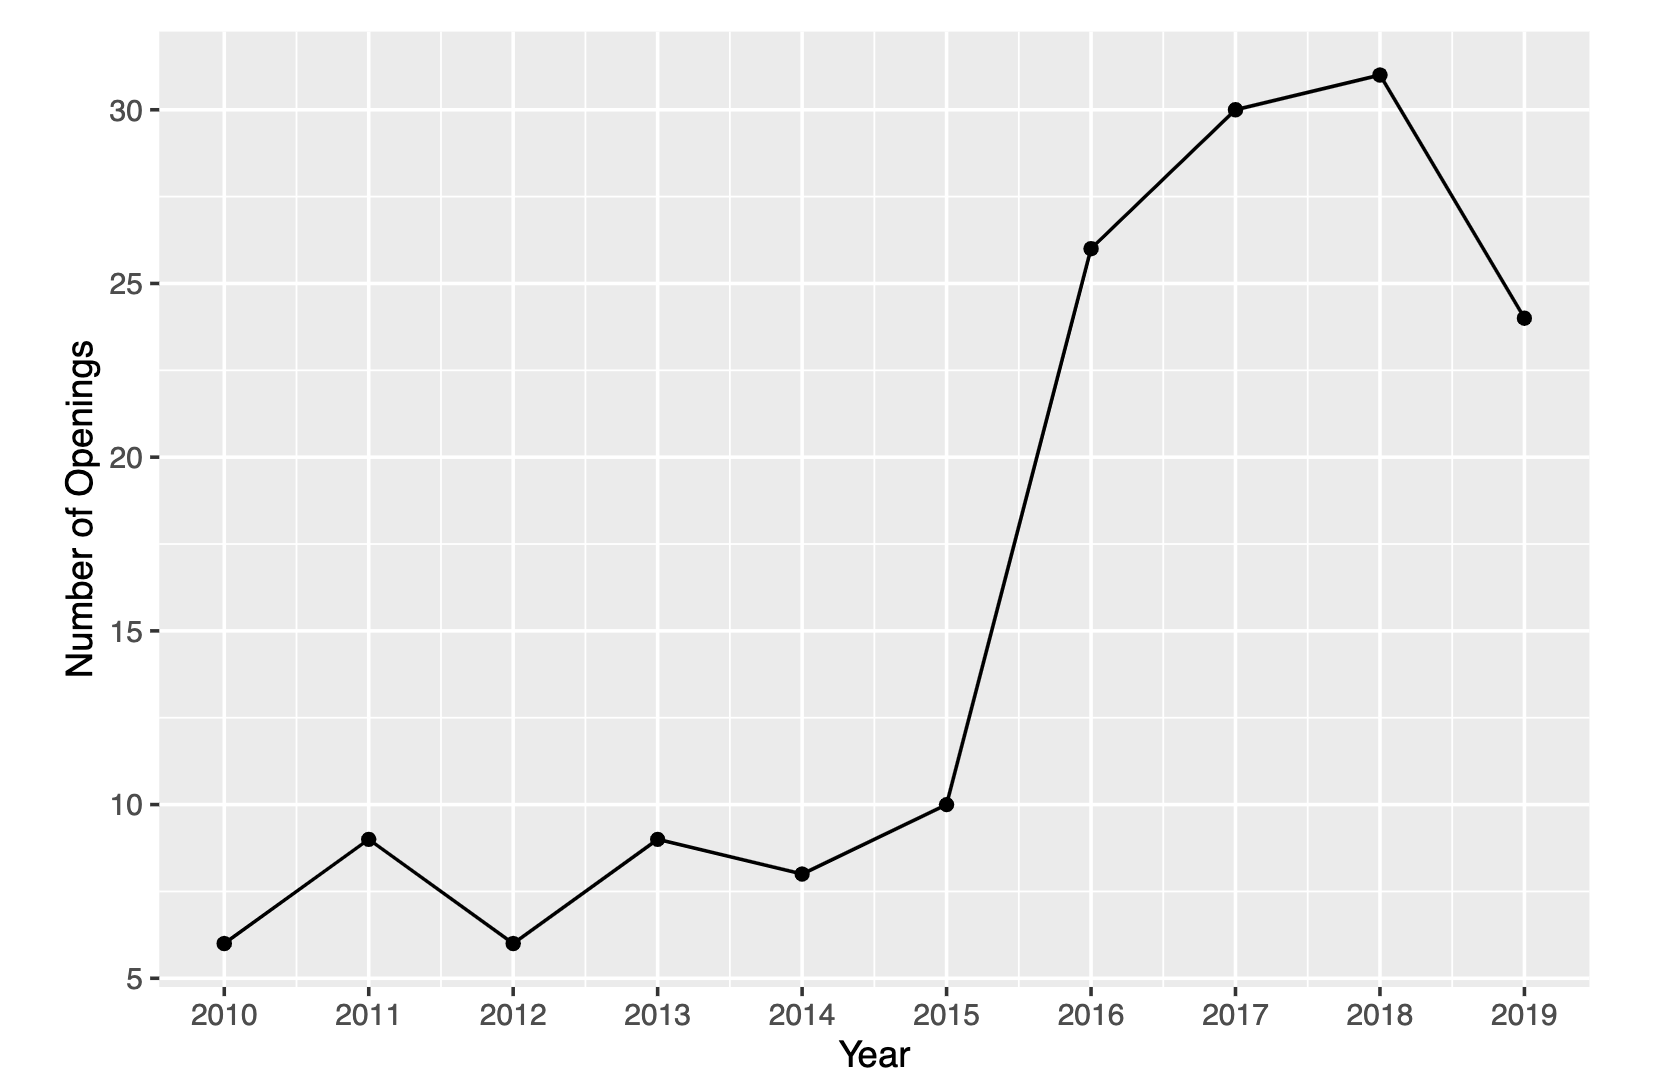
\includegraphics[width=13cm]{OPENPERYEAR.png}
\caption{Amazon Fulfillment Center openings per year from 2010-2019.}
\end{figure}

\begin{figure}[H]
\centering
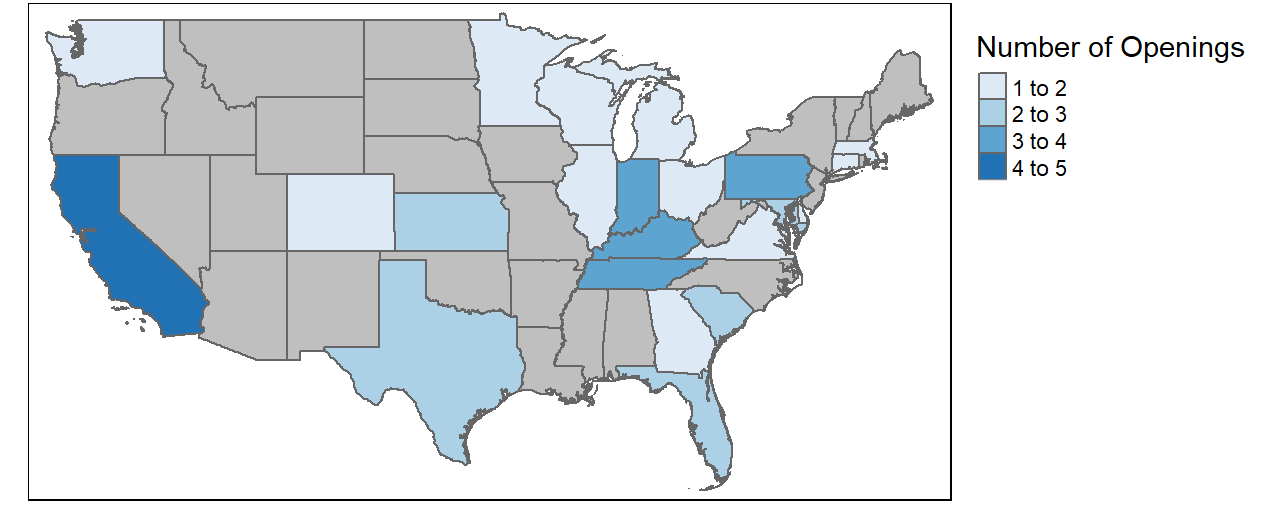
\includegraphics[width=17.5cm]{Map2Data.png}
\caption{Amazon Fulfillment Center openings per state where there were no further AFC openings 2 years before and 2 years after the initial AFC opening in the county where the initial AFC opening was located.}
\end{figure}

\subsection{Single Industry Employment Change}

\-\hspace{0.5cm} We use a simple average per period analysis to compare total industry employment, industry employment to county population ratio, and industry employment to total employment ratio for a single industry.

$$Y_{t} = \beta_0+ \beta_1*d_{t} + \epsilon_{t}$$

\begin{enumerate}
    \item $Y_{t}$ is the outcome variable measuring either industry employment to county population ratio or industry employment to total employment ratio
    \item $d_{t}$ is an indicator variable which is $1$ if the industry is in period $t = 1$, the post-treatment period, and  0 otherwise
    \item $\beta_j$ for $j\in \{0,1\}$ are regression coefficients measuring outcome variable changes 
    \item $\epsilon_{t}$ measures the error term for the industry in period $t$
\end{enumerate}

\subsection{Industry Employment Difference-in-Differences with Year Fixed-Effects}

\-\hspace{0.5cm} We use a differences-in-differences model to analyze the change in industry employment to country population ratio and industry employment to total employment ratio comparing warehouse industry employment to the industries of food manufacturing, fabricated metals manufacturing, machinery manufacturing, restaurants, and merchant wholesalers.

$$Y_{it} = \beta_1 *d_{it} + \beta_2*X_{it} + \beta_3(d_{it}*X_{it}) + \delta + \epsilon_{it}$$

The variables used are described as follows: 

\begin{enumerate}
    \item $Y_{it}$ is the outcome variable measuring either industry employment to county population ratio or industry employment to total employment ratio
    \item $d_{it}$ is an indicator variable which is $1$ if industry $i$ is in period $t = 1$, the post-treatment period, and  0 otherwise
    \item $X_{it}$ is an indicator variable which is $1$ if industry $i$ is the warehouse industry, 0 otherwise
    \item $\delta$ is our year fixed-effects
    \item $\beta_j$ for $j\in \{1,2,3\}$ are regression coefficients measuring outcome variable changes 
    \item $\epsilon_{it}$ measures error for industry $i$ at period $t$.
\end{enumerate}

\clearpage

\section{Data and Methodology for Mobility}

\-\hspace{0.5cm} Unlike the regional employment question, which may  concern itself primarily with aggregate data, determining the impact of Amazon employment on warehouse workers necessitates analysis on the individual level. To this end, the Brookings Institution graciously provided us with data scraped from online job-searching sites, particularly LinkedIn job profiles that include employment information --  including estimated income, company, start-date, and end-date -- on various workers and jobs. 

\-\hspace{0.5cm} For the purpose of this study, we consider warehouse workers to be the restrictive class of workers in the following list of tagged roles:

\begin{multicols}{2}
\begin{itemize}
    \item Package handler
    \item Delivery driver
    \item Warehouse
    \item Packer
    \item Forklift
    \item Truck driver
\end{itemize}

\columnbreak

\begin{itemize}
    \item Warehouse worker
    \item Driver
    \item Ramp agent
    \item Stockroom
    \item Transport
\end{itemize}
\end{multicols}

\-\hspace{0.5cm} While this selection certainly excludes certain classes of warehouse workers, these cohorts also held many non-warehouse roles in the same tag.

\-\hspace{0.5cm} With this list of roles, our data set had about six million observations of warehouse workers. Of these observations, approximately two hundred thousand represented workers who had ever worked at Amazon. Further, we restrict our attention to roles beginning after 2000, since the number of Amazon warehouse roles before this time is negligible, so including these data would skew income comparisons. Below are the corresponding descriptive statistics. Note that the apparent spikes in the second graph are due to people rounding their role length to the year, as they occur in 12-month increments. 

\begin{figure}[H]
\centering
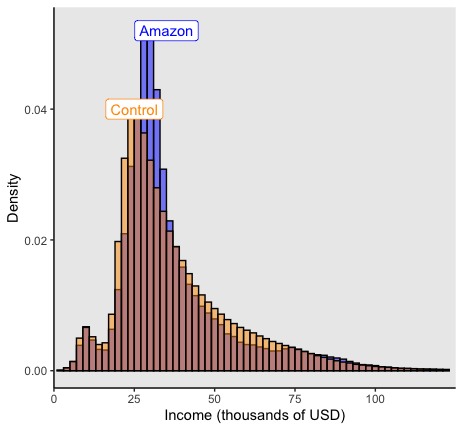
\includegraphics[width=10cm]{Rplot01.png}
\caption{Income Distribution for Amazon and non-Amazon warehouse workers}
\end{figure}

\begin{figure}[H]
\centering
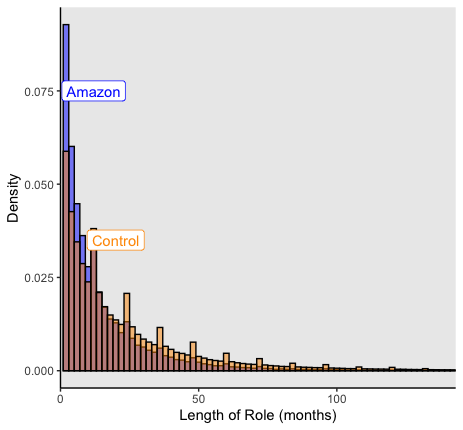
\includegraphics[width=10cm]{Rplot02.png}
\caption{Role Length Distribution for Amazon and non-Amazon warehouse workers}
\end{figure}

\begin{figure}[H]
\centering
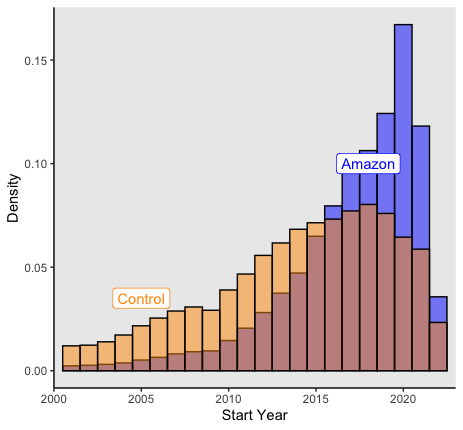
\includegraphics[width=10cm]{Rplot04.png}
\caption{Start Year Distribution for Amazon and non-Amazon warehouse workers}
\end{figure}

\-\hspace{0.5cm} The disparity between the distributions in the time of employment for Amazon and non-Amazon warehouse workers provide certain limitations in methodology for giving an answer to the mobility question. In particular, the number of observations where Amazon roles and non-Amazon roles are directly comparable in terms of start-date and role length is not sufficient to draw any statistically significant conclusions. Thus, we split our analysis of the mobility question into a two-pronged approach: 

\subsection{Mobility with Year Fixed-Effects}

\-\hspace{0.5cm} Our first model seeks to partially answer the mobility question by comparing incomes of warehouse workers who have and have not worked at Amazon following their first warehouse job. For this, we use a difference-in-differences model with year fixed-effects described in the following equation:

$$Y_{it} = \beta_0+ \beta_1 \delta_{tP_i} + \beta_2\delta_{iT} + \beta_3(\delta_{tP_i}\delta_{iT}) + \alpha_t+ \epsilon_{it}$$

The variables used are described as follows: 

\begin{enumerate}
    \item $Y_{it}$ is the income for person $i$ at time $t$ in USD.
    \item $\delta_{iT}$ is an indicator variable which is $1$ if person $i$ holds an Amazon warehouse job in our data-set and $0$ otherwise.
    \item $P_i$ is the treatment period for person $i$ which is the time range after person $i$ holds their first warehouse job
    \item $\delta_{tP_i}$ is an indicator variable which is is $1$ if $t$ is in $P_i$ and $0$ otherwise.
    \item $\alpha_t$ gives the year fixed-effect to income depending on year of $t$.
    \item $\beta_j$ for $j\in \{0,1,2,3\}$ are regression parameters measuring income for the different combinations of indicator random variables.
    \item $\epsilon_{it}$ measures error for person $i$ at time $t$.
\end{enumerate}

We present two sets of results for this methodology due to the data seen in Figures 3-5. For both sets, given the comparatively small frequency of jobs for warehouse workers who worked at Amazon beginning in 2000, we restrict the data to only look at roles beginning after the year $2000$. Additionally, due to the spike in roles for warehouse workers who have worked at Amazon in 2020 and differences in macroeconomic trends due to the COVID-19 pandemic, we present one data set which includes data from this period (March 2020 onwards) and one which excludes it. 



\subsection{Mobility with Manually Computed Fixed-Effects}

\-\hspace{0.5cm} The second model intends to delineate the effect that Amazon employment has on blue-collar worker mobility, again using a differences in differences specification. Here, the exception is that the year fixed effects vector is excluded, and is incorporated manually by iterating the model multiple times with different fixed start and end dates. This approach also allows for the assessment of mobility across time periods. Notably, the effects of the COVID-19 pandemic can now be examined directly by altering the start and end dates for the model. We describe the model as follows:

$$Y_{it} = \beta_0 + \beta_1\delta_{t} + \beta_2\delta_{iT} + \beta_3(\delta_t\delta_{iT}) + \epsilon_{it}$$

The variables used are described as follows: 

\begin{enumerate}
    \item $Y_{it}$ is the income for person $i$ at time $t$ in USD.
    \item $\delta_{iT}$ is an indicator variable which is $1$ if person $i$ holds an Amazon warehouse job in our data-set and $0$ otherwise.
    \item $\delta_{t}$ is an indicator variable which is is $0$ if $t$ is in the pre-treatment time period and $0$ if in the post-treatment time period.
    \item $\beta_j$ for $j\in \{0,1,2,3\}$ are regression parameters measuring income for the different combinations of indicator random variables.
    \item $\epsilon_{it}$ measures error for person $i$ at time $t$.
\end{enumerate}

The pre-treatment and post-treatment time periods are hyperparameters in this model, and the results ranging across the possible choices for these parameters are displayed below (LINK). In addition to the regression coefficient results, we display graphics depicting the p-values, the number of observations, and the average time spent in the role for each combination of hyperparameters our model is run on.

\section{Notes on the Difference-in-Differences Framework}
\-\hspace{0.5cm} In order to investigate both regional employment and mobility questions described above while considering unobserved confounders, we employ a fixed-effects difference-in-differences specification (Angrist, 2008). Such models are used in observational settings where exchangeability cannot be assumed between the treatment and control groups. There is a less strict exchangeability assumption in that the unobserved differences between treatment and control groups are parallel over time. Thus, the D-in-D framework is useful given these data and the fact that randomization of treatment/control status is not possible on the individual level.

\-\hspace{0.5cm} With regard to our regional employment model, we compare industries that are closely related in their makeup of low-income employment and appeal to low-income individuals. This choice of industries is a result of wanting to specifically isolate the employment movement in industries that are largely dependent on the labor provided by low-income individuals, as these are the individuals that are drawn to work in Amazon Fulfillment Centers. In constructing our mobility models, we accessed longitudinal/panel data that allowed us to analyze observations of the same individuals (Amazon workers) over time. This approach is aimed at removing omitted variable bias in post-intervention period comparisons between the treatment and control groups, which could be due to permanent intrinsic differences between the groups or exogenous trends due to other causes of the outcome. Before proceeding with analysis of these data, we state the main assumptions which must hold in order to estimate any causal effect: exchangeability, positivity, and Stable Unit Treatment Value Assumption (SUTVA). 
\begin{enumerate}
    \item The intervention is unrelated to outcomes in the absence of treatment (allocation of treatment was not determined by outcome).
    \item Treatment and control groups have Parallel Trends in outcome (see below).
    \item Composition of treatment and control groups is stable for a repeated cross-sectional design.
    \item The potential outcomes for any unit do not vary with the treatments assigned to other units (no spillovers).
\end{enumerate}
\-\hspace{0.5cm} The parallel trends assumption is the most critical of the above four to ensure internal validity of the Difference-in-Differences model, and as such, is the most difficult to fulfill. This assumption requires that in the absence of treatment, the difference between groups is constant over time. Having been unable to conduct statistical tests to ensure this assumption is met, we use visual inspection of our observations over several points in time. We recognize that, in our analyses that include data points from a larger time interval (10-20 years), it is possible that the Parallel Trends assumption may not hold. With regard to our regional employment models, overall economic trends in counties allow for the assumption that employment growth in industries would remain constant over time, allowing us to reasonably assume the parallel trends assumption is satisfied. With regard to our mobility models, our approach allows us to use individual data with comparison groups starting at different levels of the outcome (income), since this framework focuses on relative inter-temporal change rather than absolute levels of the outcome variables. 

\section{Results}


\subsection{Analysis of Regional Employment}

\-\hspace{0.5cm} Descriptive statistics for the variables of average warehouse employment, average total employment, and average county population are included in Table 1. The average warehouse employment in period 0 was 2551 warehousing employers compared to 3718 in period 1, a 45\% increase. In addition, we find a 5.2\% increase in average total employment from period 0 to period 1 and a 2.6\% increase in average county population from period 0 to period 1. Figure 7 presents the average percent change in employment for each industry from period 0 to period 1.

\begin{table}[H]
\centering
\begin{tabular}[H]{lcccccc}
\toprule
&Min&Max&Range&Median&Mean&SD\\
\midrule
A1&54&15429&15375&1529&2550.89&3134.34\\
A2&302&19877&19575&2992&3717.86&3548.4\\
B1&15092&3932904&3917812&115433&298321.82&643026.86\\
B2&18342&3869073&3850731&128534&313993.66&638439.47\\
C1&57915&10040072&9982157&391036&745591.63&1608428.1\\
C2&63033&10073906&1001087&3391742&765314.32&1616917.79\\
\bottomrule
\end{tabular}
\caption{Descriptive statistics for the variables of warehouse employment per county before openings (A1), warehouse employment per county after openings (A2), total employment per county before openings (B1), total employment per county after openings (B2), county population before openings (C1), and county population after openings (C2).}
\end{table}%

\-\hspace{0.5cm} Table 2 contains the results for our single industry employment change regressions. For each of the 9 industries, we find the change in industry employment to county population ratio and the change in industry employment to total employment ratio. We see that for the warehouse employment to county population ratio (A1), there is a 0.4 percentage point increase in the ratio, and for the warehouse employment to total employment ratio, there is a 1.6 percentage point increase in the ratio. From all 9 industries of analysis, warehouse employment had both the largest increase in industry employment to county population ratio and industry employment to total employment ratio. The second largest increase in county population ratio and total employment ratio was construction with a 0.3 percentage point increase and 0.6 percentage point increase, respectively. Figure 6 presents the change in warehousing employment and its corresponding ratios. Figures 13-21, in the appendix, display the change in industry employment and its corresponding ratios for the industries of construction, food manufacturing, fabricated metals manufacturing, machinery manufacturing, freight trucking, restaurants and other eating places, repair and maintenance, services to buildings and dwellings, and merchant wholesalers. Machinery manufacturing was the only industry that saw a decrease in industry employment to county population ratio, with a decrease of 0.01 percentage points. The industries of fabricated metals manufacturing and repair/maintenance saw a decrease in their industry employment to total employment ratios, with a decrease of 0.04 and 0.05 percentage points, respectively.  Figures 8 and 9 display the change in county population ratios and total employment ratios for each industry, respectively.  

\begin{table}[H]
\centering
\begin{tabular}[H]{lcccccc}
\toprule
&Treatment Coef.&Std. Error&p-value&Conf. Interval\\
\midrule

A1&0.00497 &0.0027&0.0682&[-0.0004, 0.0103]\\
A2&0.0161 &0.0073&0.0327 (*) &[0.0014, 0.0308]\\
B1&0.0034 &0.0015&0.0287 (*)&[0.0004, 0.0064]\\
B2&0.006&0.0047&0.2068&[-0.0034, 0.0154]\\
C1&0.0021 &0.0042&0.6164&[-0.0063, 0.0106]\\
C2&0.0004 &0.0107&0.9731&[-0.0211, 0.0218]\\
D1&0.0001 &0.0007&0.8547&[-0.0012, 0.0014]\\
D2&-0.0004 &0.0016&0.7841&[-0.0036, 0.0027]\\
E1&-0.0001 &0.0007&0.8466&[-0.0015, 0.0012]\\
E2&0.00005 &0.0021&0.9788&[-0.004, 0.0042]\\
F1&0.0006 &0.0011&0.59&[-0.0015, 0.0027]\\
F2&0.0009 &0.0027&0.7454&[-0.0045, 0.0062]\\
G1&0.0025 &0.0016&0.1145&[-0.0006, 0.0056]\\
G2&0.0017 &0.0056&0.762&[-0.0096, 0.013]\\
H1&0.0002 &0.0004&0.655&[-0.0007, 0.0011]\\
H2&-0.0005 &0.0019&0.8058&[-0.0043, 0.0034]\\
I1& 0.0006 &0.0008&0.3952&[-0.0009, 0.0022]\\
I2&0.0007 &0.0014&0.6229&[-0.0021, 0.0035]\\
J1&0.0008 &0.0017&0.6288&[-0.0026, 0.0042]\\
J2&0.0002 &0.003&0.9451&[-0.0057, 0.0061]\\
K&0.0224& 0.0229& 0.3301& [-0.0232, 0.068]\\
\bottomrule
\end{tabular}
\caption{OLS results for the different employment industries analyzed. For each industry, we analyze both the employment-to-county population ratio (1) and the employment-to-total country employment ratio (2). Industries include: warehousing (A), construction (B), food manufacturing (C), fabricated metals manufacturing (D), machinery manufacturing (E), freight trucking (F), restaurants and other eating places (G), repair and maintenance (H), services to buildings and dwellings (I), merchant wholesalers (J), and lastly total employment (K).}
\end{table}%

\begin{figure}[H]
\centering
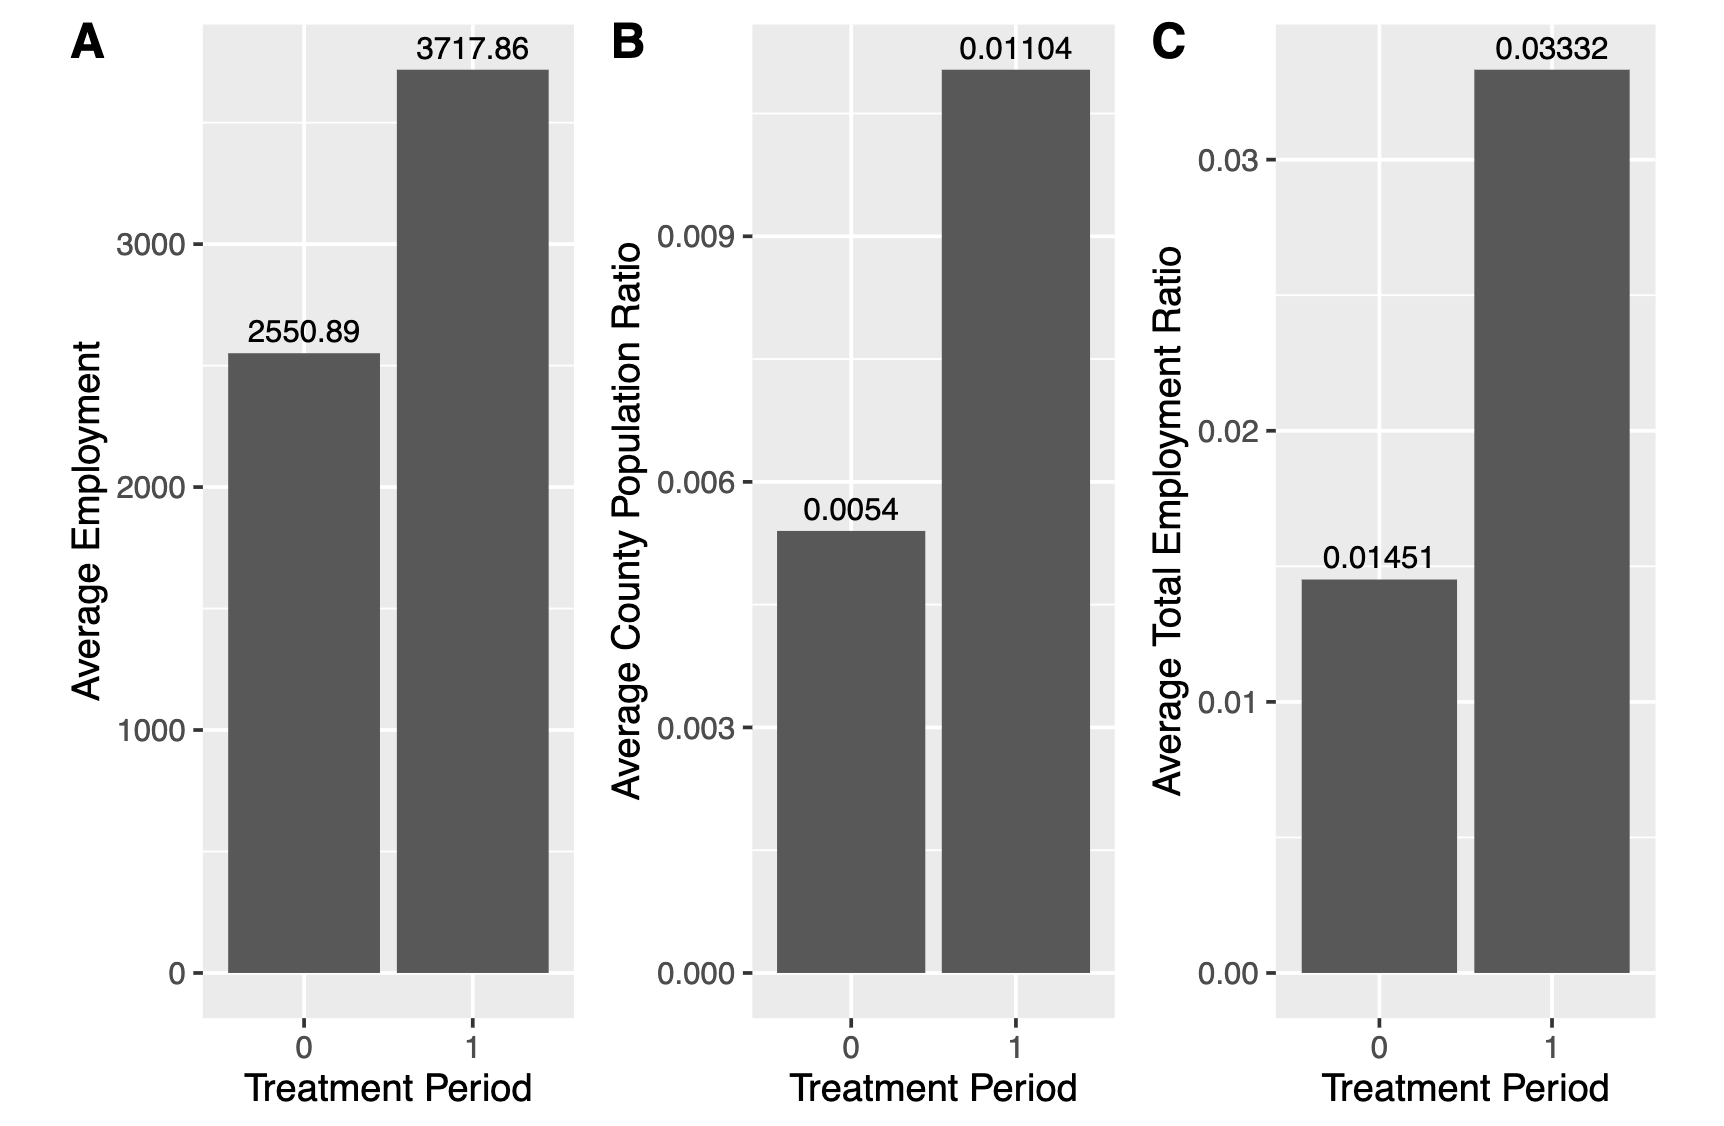
\includegraphics[width=15cm]{WH.png}
\caption{Warehouse employment 2 years before and 2 years after Amazon Fulfillment Center openings}
\end{figure}


\-\hspace{0.5cm} Table 3 includes the results for our difference-in-differences model on industry employment to county population ratio. We find that there is an increase in industry employment to county population ratio for warehousing as compared to our comparison industries of 1.66 percentage points. This coefficient comes with a p-value of 0.087, meaning we cannot reject the null hypothesis of there being no relationship. 

\begin{table}[H]
\centering
\begin{tabular}[H]{lcccccc}
\toprule
&Coef.&Std. Error&p-value&Conf. Interval\\
\midrule
$\beta_1$&0.00135&0.0051&0.7923&[-0.0087, 0.0114]\\
$\beta_2$&-0.0339&0.0048&0.0000&[-0.0434, -0.0244]\\
$\beta_3$&0.0166&0.0097&0.0871&[-0.0024, 0.0356]\\
\bottomrule
\end{tabular}
\caption{Differences-in-Differences results for industry employment to county population ratio.}
\end{table}%

\-\hspace{0.5cm} Table 4 includes the results for our difference-in-differences model on industry employment to county population ratio. We find that there is an increase in industry employment to total employment ratio for warehousing as compared to our comparison industries of 0.42 percentage points. This coefficient comes with a p-value of 0.226, meaning we cannot reject the null hypothesis of there being no relationship. 

\begin{table}[H]
\centering
\begin{tabular}[H]{lcccccc}
\toprule
&Coef.&Std. Error&p-value&Conf. Interval\\
\midrule
$\beta_1$&0.0014&0.0019&0.4492&[-0.0023, 0.0051]\\
$\beta_2$&-0.012&0.0022&0.0000&[-0.0162, -0.0077]\\
$\beta_3$&0.0042&0.0035&0.2261&[-0.0026, 0.011]\\
\bottomrule
\end{tabular}
\caption{Differences-in-Differences results for industry employment to total employment ratio.}
\end{table}%


\begin{figure}[H]
\centering
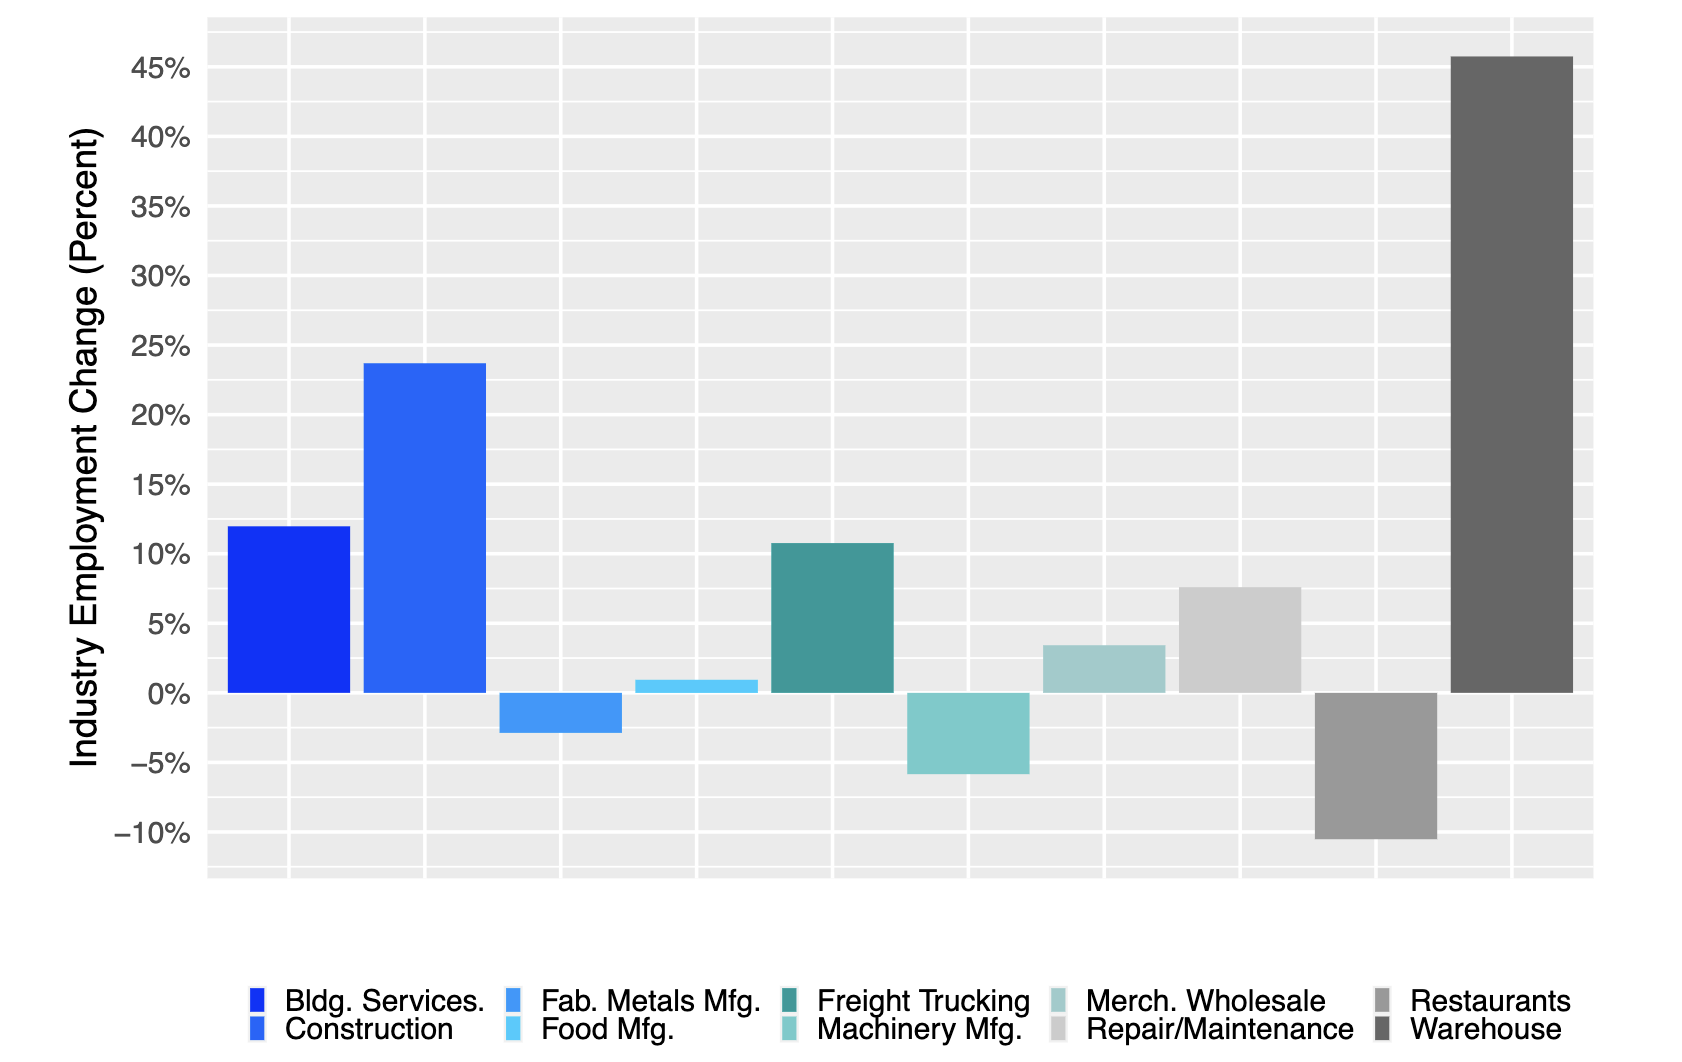
\includegraphics[width=15cm]{EMP.png}
\caption{Change in Employment Per Industry}
\end{figure}


\begin{figure}[H]
\centering
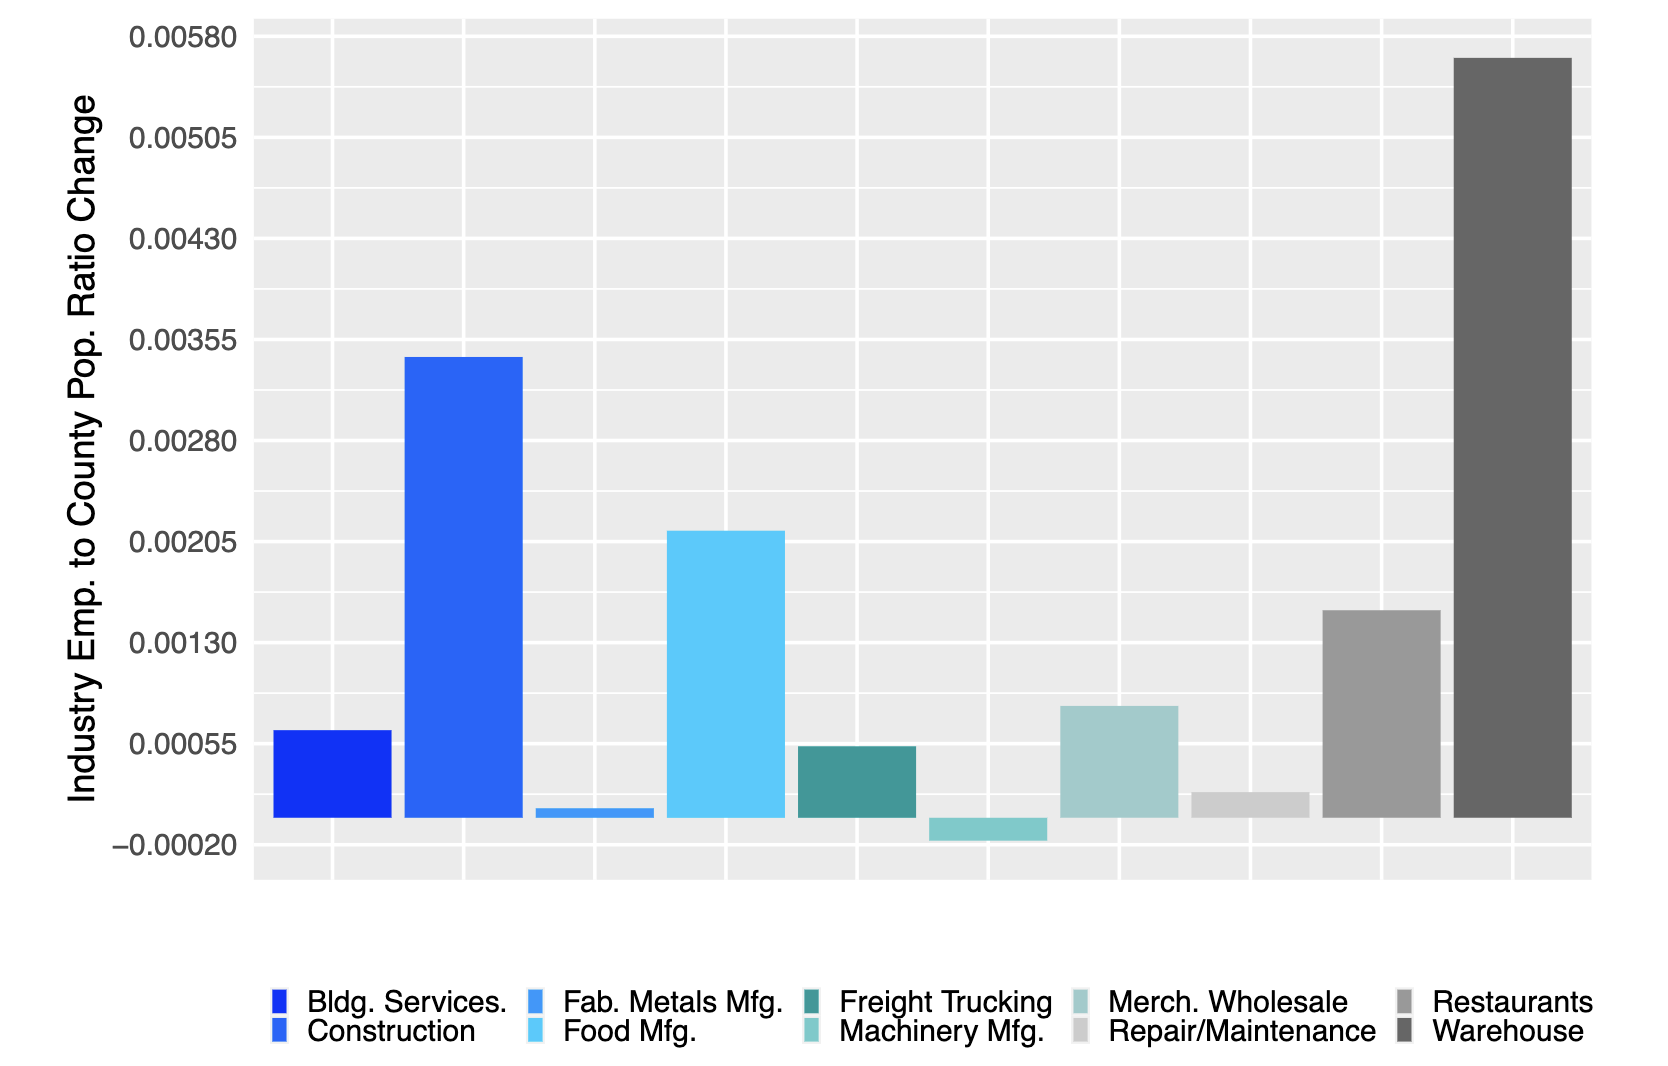
\includegraphics[width=15cm]{CTEMP.png}
\caption{Change in Industry Employment to County Population}
\end{figure}

\begin{figure}[H]
\centering
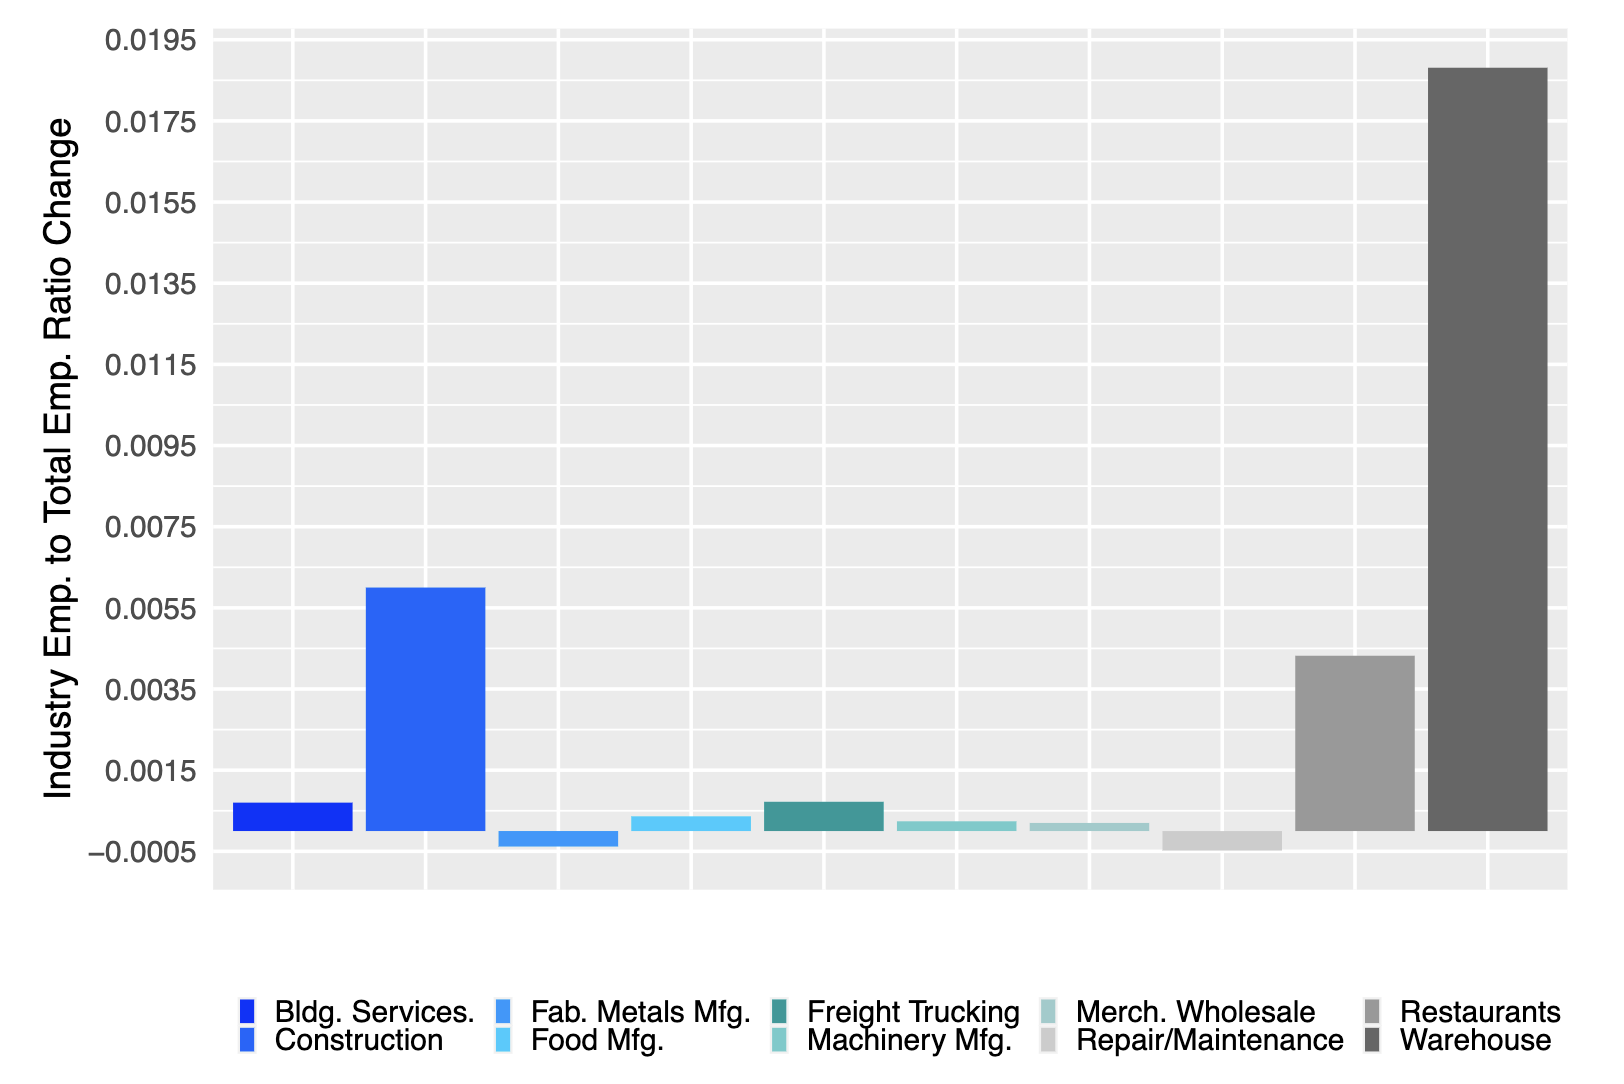
\includegraphics[width=15cm]{TOTEMP.png}
\caption{Change in Industry Employment to Total County Employment}
\end{figure}

\subsection{Discussion of Regional Employment}

\-\hspace{0.5cm} As expected, we find a significant increase in average warehouse employment from period 0 to period 1. With the introduction of Amazon Fulfillment Centers, the warehousing industry employment increased, indicating an increase in new warehousing jobs, a partial fulfillment of Amazon's promise of net job growth. However, with this promise comes an implicit assumption that the labor makeup of adjacent industries should not change, i.e. that other industries' employment should not decrease as a result of the introduction of Amazon Fulfillment centers. When analyzed in isolation, warehouse employment to total population ratio rose significantly, with a 1.6 percentage point increase. This displays the idea that warehousing is taking a larger share of the labor supply in these counties. Once again, this in itself does show that new warehouse jobs are introduced to a county. However, when analyzing the average total employment to county population ratio change from period 0 to period 1, we find a non-significant increase, so we cannot deduce that new net jobs were introduced to the counties. From our difference-in-differences model, we find that the increase in industry employment ratios for warehousing is not significantly different from the increase in our comparison industry ratios. If new net jobs were to be introduced by the AFC openings, we would expect the increase in total employment and county population ratios for warehousing to be significant as compared to our comparison industries -- a significant increase would indicate that an introduction of new warehouse jobs would be the result of new net jobs being introduced to the county as a whole instead of a change in the makeup of the labor force.

\-\hspace{0.5cm} It is noteworthy to point out potential flaws in our methodology. In our single industry employment analysis, we simply take an average per period of the different employment ratios. We cannot definitively say that the Amazon Fulfillment Center openings were the cause for any changes we reported since we take these averages across a 4 year period, leaving room for many exogenous events to take place that can alter the results produced. Such shocks include, but are not limited to, new government regulations, business cycle fluctuations, etc. We can only confidently report these findings as observed changes that are present when analyzing a time period before fulfillment center openings and a time period after the openings. With regard to our difference-in-differences models, given our small sample size of counties, it is again difficult to draw strong conclusions from our results. In addition, our comparison group, consisting of the industries of food manufacturing, fabricated metals manufacturing, machinery manufacturing, restaurants, and merchant wholesalers, are likely not entirely representative of all industries present in a county from which Amazon can lure low-income workers. As a result, we do not see a significant difference in the increase between the employment ratios of warehousing and the comparison industries given that it is likely that other industries outside of these had significant changes that we either did not analyze or did not account for. \\


\subsection{Analysis of Mobility with Year Fixed-Effects}

First Model Specification:

$$Y_{it} = \beta_0+ \beta_1 \delta_{tP_i} + \beta_2\delta_{iT} + \beta_3(\delta_{tP_i}\delta_{iT}) + \alpha_t+ \epsilon_{it}$$

Regression Results:

\begin{table}[H]
\centering
\begin{tabular}[H]{lcccccc}
\toprule
&Coef.&Std. Error&t-value&p-value &\\
\midrule
$\beta_0$& 55305.34 & 60.57 & 913.05 & $<$0.001***\\
$\beta_1$& -1069.99 & 22.32 & -47.94 & $<$0.001***\\
$\beta_2$& -3191.57 & 95.14 & -33.55 & $<$0.001***\\
$\beta_3$& -1315.05 & 113.23 & -11.61 & $<$0.001***\\
\bottomrule
\end{tabular}
\caption{Differences-in-differences results for Model One including data from the COVID-19 Pandemic}
\end{table}%


\begin{table}[H]
\centering
\begin{tabular}[H]{lcccccc}
\toprule
&Coef.&Std. Error&t-value&p-value &\\
\midrule
$\beta_0$& 47557.13 & 83.60 & 568.888 & $<$0.001***\\
$\beta_1$& -612.52 & 24.07 & -25.448 & $<$0.001***\\
$\beta_2$& -2767.07 & 115.58 & -23.941 & $<$0.001***\\
$\beta_3$& -1179.04 & 137.99 & -8.544 & $<$0.001***\\
\bottomrule
\end{tabular}
\caption{Differences-in-differences results for Model One excluding data from the COVID-19 Pandemic}
\end{table}%

\-\hspace{0.5cm} In interpreting these results plainly, $\beta_0$ gives the average income of people who will ever hold a warehouse job before their first warehouse role. $\beta_1$ gives the average change in income upon holding this first warehouse role. $\beta_2$ gives the difference in income between warehouse workers who will ever hold an Amazon role and other warehouse workers before their first warehouse job. Finally, $\beta_3$ gives the average change in income upon holding warehouse roles for those who will eventually work at Amazon relative to the change experienced by other workers who will hold a warehouse role. 

\-\hspace{0.5cm} In summary, these results suggest that those who will hold Amazon warehouse roles are likely to lose income upon entering warehouse roles as compared to the average warehouse workers, by an average of $\$1,200-\$1,300.$

\-\hspace{0.5cm} We include the results from both time periods (including and excluding COVID-19) as the pandemic saw a sharp uptick in Amazon employment which can be seen in the distribution of start dates. Thus, since this increase carries very likely differences in trends between Amazon and non-Amazon roles, the parallel trends assumption holds with more generality for the time period excluding the pandemic. Given that our model used year-fixed effects, including this time period only slightly shifted the results observed. 

\subsection{Analysis of Mobility with Manually Computed Fixed-Effects}
\begin{figure}[H]
    \centering
    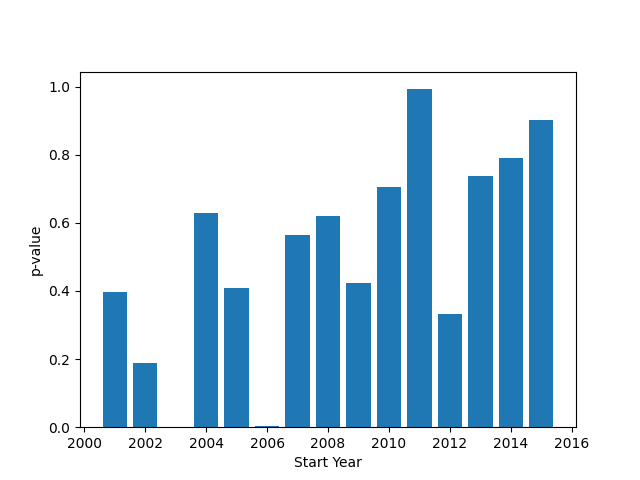
\includegraphics[width=13cm]{p-values_mob2.png}
    \caption{p-values for given Hyperparameters in Mobility Model Two}
\end{figure}


\-\hspace{0.5cm} As seen in the above figure, the significance of the regression with manually computed fixed effects was not enough to make conclusive claims. The only starting year with significant results was 2006, and Figure 11 shows there was significance in that the results implied Amazon work did improve mobility for workers starting at this time. Possible reasons for this result may be effects from the 2008 recession, but this is unlikely as we do not see similar results in similar years (2005,2007).

\-\hspace{0.5cm} A possible explanation for the difference between the two models is that in each starting time frame, there are no significant results as the sample sizes are smaller (Figure 12). However, the full regression leads to significant results due to the size of the data set. Importantly, even if there are significant results in the general regression, there is notable variance in mobility differences between different starting years. As we discuss later, the nature of Amazon employment is likely fundamentally different from general warehouse employment, and it is difficult to extend these mobility results to a general claim.

\subsection{Discussion of Mobility}

\-\hspace{0.5cm} The findings differed between the two models both in significance and in interpretation. Model one had statistically significant results implying that warehouse work decreased mobility for workers who would eventually be employed at Amazon when compared to the mobility of general warehouse workers. Model two had insignificant results with varying results across time. Overall, the results from the two different models are unable to definitively confirm any conclusions, primarily due to the differences in the employment type, notably the average time spent in a role. Further separations, such as the average start date, exacerbate these difficulties.

\-\hspace{0.5cm} There is significant difficulty in attempting to compare these two types of employment, as temporary forms of employment will attract different types of individuals, as well as lead individuals into and out of new roles quickly, be they more or less mobile. Any attempt to compare the two would need to account for these effects in some manner, where our models had, as an assumption, that individual fixed effects were constant.

\-\hspace{0.5cm} In practice, this means that the results for the first model, which show a definitive decrease in income between the treatment group and control group after the first warehouse job for every individual, cannot be taken as necessarily indicative of the overall effect of Amazon employment on individuals. In particular, since individuals who eventually work at Amazon have a longer average role length, it is possible that the effect described is caused by these individuals' predispositions to shorter roles rather than Amazon employment. This is further supported by the conclusions of model two as comparisons between Amazon and non-Amazon workers for fixed time lengths yield no conclusive evidence. However, at least some of the statistical insignificance of the results of the second model are due to the small number of observations needed to compare long-term roles at Amazon Warehouses and non-Amazon Warehouses due to the rise of Amazon roles and their comparatively shorter tenures.

\-\hspace{0.5cm} However, while the definitive conclusions that can be drawn about the exact effect of Amazon employment are limited, our study does suggest that employment at Amazon does not increase the mobility of warehouse workers. 


\section{General Discussion}
\begin{text}
\-\hspace{0.5cm} We now explore the interconnected nature of our two research questions and their implications for policy. First, our findings indicate that while the introduction of AFCs did not significantly increase total county employment, it did lead to an increase in warehouse employment, altering the composition of labor sectors in each respective region. This indicates that AFCs may have contributed to a reallocation of regional labor forces -- which is likely due to the displacement of jobs in non-warehousing industries and the tendency of large corporations such as Amazon to draw workers out of other industries to fill warehouse positions. 

\-\hspace{0.5cm} State and local policymakers seeking maximum long-term benefits can consider several strategies in light of these findings. Given that introducing AFCs has led to an increase in warehouse employment, policymakers can focus on improving the hiring process in this sector. This could include collaboration with large employers to ensure transparency of job responsibilities, benefits, and working conditions, rather than over-relying on temporary work arrangements. In addition, several strategies could be implemented to support workers through their transitions between industries. According to the OECD, worker's compensation programs that provide medical care, cash benefits, or job training can foster strong job-worker matches and ensure that workers can continue to upgrade their skills. Such training and reskilling programs can offer much-needed support to those workers who are  displaced by the expansion of the warehouse sector. 

\-\hspace{0.5cm} We suggest that the primary aim of worker quality enhancement programs is to ensure that the growth in warehouse employment leads to meaningful economic mobility for workers.  As such, this can involve providing targeted training programs for transitioning or established warehouse workers. Becker's seminal Human Capital theory emphasizes the importance of education and skill development in enhancing workers' productivity and earnings potential (Becker \& Tomes, 1979). Further, the theory states that an individual will engage in training when the present discounted value of its benefits exceeds the cost of training. When a single training opportunity is available to an individual, and if the individual has reasonable foresight of the future, policies can be geared toward the direction of providing training incentives to workers. We recognize that workers may be hesitant to participate in such programs due to financial or time constraints, but the behavioral literature suggests that financial incentives (i.e. grants, scholarships, and cost-coverage by employers) can make these programs significantly more accessible (Babcock et al. 2012). Another simple intervention could be the addition of career advancement opportunities -- clear pathways which link training program participation to promotions or other opportunities. If workers are made aware that participating in quality enhancement programs may directly contribute to their career progression, they may be more likely to participate in such programs, to begin with. In order to support newly transitioned workers, employers should ensure that they are properly recognized for their investment into skill-building exercises. In practice, this could include mentorship programs and consistent support throughout the training process. Our analysis of qualitative sentiment surveys suggests that several Amazon Warehouse workers lack the confidence to invest in their professional development, so such support and recognition could indirectly increase workers' future employability and encourage them to take advantage of the opportunities available. 

\-\hspace{0.5cm} Finally, having understood that the employment effects generated by Amazon Fulfillment Centers may have significant implications for the longer-term mobility potential of individual warehouse employees, we discuss urban revitalization efforts -- critical policy changes that can increase the welfare of regional labor markets and their constituent workers. Specifically, by discussing business investment in existing, underutilized infrastructure, we can better comprehend the broader economic implications of our findings.

\-\hspace{0.5cm} A vast literature led by Davis \& Whinston's 1961 article on the Economics of Urban Revival implies that there are several general equilibrium effects related to urban renewal. In relation to the present study, it is apparent that an influx of warehouse jobs leads to changes in the supply and demand of labor, and as a consequence, drastic changes in the employment levels of particular sectors. A general equilibrium lens can help us assess the regional and individual externalities that arise from warehousing growth. Since we see that the promised positive spillovers of AFCs (such as job growth) may be unfulfilled, we wonder whether targeted policy measures can lead to better outcomes in sector and regional economies. For example, instead of providing tax incentives for the establishment of Amazon Warehouses, local governments can provide financial incentives for investment in underutilized infrastructure. A recent but distant example of this is the establishment of the High Line in New York City's Meatpacking District, a previously underused area with minimal economic activity and social vitality. Conveniently, these widely studied infrastructure reuse projects can be adapted to fit the sustainability agendas of governments ((Viguie \& Hallegatte, 2014)). Policymakers can also support the development of affordable housing so as to prevent the displacement of vulnerable worker populations in light of the growing warehouse sector. 

\-\hspace{0.5cm} These advancements, although difficult to implement at scale, could inform more holistic urban revitalization strategies and address the simultaneous effects of warehouse employment on regional labor markets, the distribution of job opportunities, and the mobility potential of the individual worker. 

\end{text}

\clearpage


\section{References}
\begin{center}
\begin{enumerate}
 \item Department of Labor, Occupational Safety and Health Administration, “US Department of Labor Finds Amazon Exposed Workers To Unsafe Conditions, Ergonomic Hazards at Three Warehouses," 2022, Washington, DC
 \item Department of Labor, Bureau of Labor Statistics, Warehousing and Storage,  NAICS Report 493, 1994-2023, Raw Data, Washington, DC
 \item Rydstrom, Klara, Kirstina Johansson, and Jennie Jackson. “A Systematic Review of Work Organization, Work Environment, and Employment Conditions in Warehousing in Relation to Gender and Race/Ethnicity," Annals of Work Exposures and Health, 67, no. 4 (January 30, 2023). https://academic.oup.com/annweh/article/67/4/430/7010370. 
 \item Jones , Janelle, and Ben Zipperer. “Unfulfilled Promises: Amazon Fulfillment Centers Do Not Generate Broad-Based Employment Growth.” Economic Policy Institute. Accessed May 13, 2023. https://www.epi.org/publication/unfulfilled-promises-amazon-warehouses-do-not-generate-broad-based-employment-growth/. 
 \item Warehouse Workers for Justice. “Bad Jobs in Goods Movement.” Center for Urban Economic Development at the University of Illinois at Chicago. Accessed May 13, 2023. \\ https://www.ww4j.org/uploads/7/0/0/6/70064813/badjobsgoodsmovement.pdf. 
 \item Gutelius, Beth, and Nik Theodore. “The Future of Warehouse Work: Technological Change in the U.S. Logistics Industry.” UC Berkeley Labor Center, January 17, 2021. \\ https://laborcenter.berkeley.edu/future-of-warehouse-work/. 
 \item Fritsch, M., and Schindele, Y. (2011). “The contribution of new businesses to regional employment-an empirical analysis." Econ. Geogr. 87, 153–180. doi: 10.1111/j.1944-8287.2011.01113
 \item Becker, Gary S., and Nigel Tomes. “An Equilibrium Theory of
the Distribution of Income and Intergenerational Mobility.” Journal of Political Economy 87, no. 6 (1979): 1153–89. http://www.jstor.org/stable/1833328.
 \item Chetty, Raj, Nathaniel Hendren, Patrick Kline,
Emmanuel Saez, and Nicholas Turner. 2014. “Is the United States Still a Land of Opportunity? Recent Trends in Intergenerational Mobility.” American Economic Review, 104 (5): 141-47. DOI: 10.1257/aer.104.5.14
 \item Reese, Ellen, Alexander Scott. 2019. “Warehouse Employment as a Driver of Inequality in the Inland Empire: The Experiences of Young Amazon Warehouse Workers." University of California at Berkeley. Othering \& Belonging Institute.
 \item De Lara, Juan. 2013. “Warehouse Work: Path to the Middle Class or Road to Economic Insecurity?" USC Program for Environmental and Regional Equity: 1-8.
\item Angrist, J. D., and Jorn-Steffen Pischke. 2008. Mostly Harmless Econometrics. Princeton, NJ: Princeton University Press.
 \item OECD (2022), Supporting transitions and securing jobs: Social dialogue shaping a stronger recovery from the pandemic, https://www.oecd.org/coronavirus/policy-responses/supporting-transitions-and-securing-jobs-social-dialogue-shaping-a-stronger-recovery-from-the-pandemic-83b6b310/
 \item Becker, Gary S. “Investment in Human Capital: A Theoretical Analysis.” Journal of Political Economy 70, no. 5 (1962): 9–49. http://www.jstor.org/stable/1829103. 
 \item Babcock, L., Congdon, W.J., Katz, L.F. et al. 2012. “Notes on behavioral economics and labor market policy." IZA J Labor Policy 1, 2 (2012). https://doi.org/10.1186/2193-9004-1-2
 \item Davis, Otto A., and Andrew B. Whinston. “The Economics of Urban Renewal.” Law and Contemporary Problems 26, no. 1 (1961): 105–17. https://doi.org/10.2307/1190601.
 \item Viguie, V.; Hallegatte, S.. 2014. “Urban Infrastructure Investment and Rent-Capture Potentials." Policy Research Working Paper; No. 7067. © World Bank Group, Washington, DC. http://hdl.handle.net/10986/20513
\end{enumerate}  
\end{center}

\clearpage

\section{Appendix}

\begin{table}[H]
\centering
\begin{tabular}[H]{lcc}
\toprule
State&Number of Openings\\
\midrule
California	&22\\
Texas	&17\\
Pennsylvania	&12\\
New Jersey	&12\\
Illinois	&10\\
Florida	&8\\
Arizona	&7\\
Ohio	&7\\
Indiana	&6\\
Washington	&5\\
Nevada	&5\\
Georgia	&4\\
Maryland	&4\\
Tennessee	&4\\
South Carolina	&4\\
Kentucky	&3\\
Michigan	&3\\
Utah	&3\\
Virginia	&3\\
Oregon	&3\\
Wisconsin	&2\\
North Carolina	&2\\
Kansas	&2\\
Connecticut	&2\\
Colorado	&2\\
Oklahoma	&1\\
New York	&1\\
Mississippi	&1\\
Minnesota	&1\\
Massachusetts	&1\\
Delaware	&1\\
Missouri	&1\\
\bottomrule
\end{tabular}
\caption{Number of Amazon Fulfillment Center Openings by state from 2010-2019.}
\end{table}%

\begin{table}[H]
\centering
\begin{tabular}[H]{lcc}
\toprule
State&Number of Openings\\
\midrule
California	&5\\
Pennsylvania	&3\\
Indiana	&3\\
Kentucky	&3\\
Tennessee	&3\\
New Jersey	&2\\
Texas	&2\\
Maryland	&2\\
Florida	&2\\
Kansas	&2\\
South Carolina	&2\\
Colorado	&1\\
Illinois	&1\\
Delaware	&1\\
Michigan	&1\\
Ohio	&1\\
Connecticut	&1\\
Washington	&1\\
Wisconsin	&1\\
Georgia	&1\\
Virginia	&1\\
Massachusetts	&1\\
Minnesota	&1\\
\bottomrule
\end{tabular}
\caption{Number of Amazon Fulfillment Center openings by state from 2011-2017 in counties where there were no more AFC openings two years before and after an initial AFC opening.}
\end{table}%

\begin{figure}
    \centering
    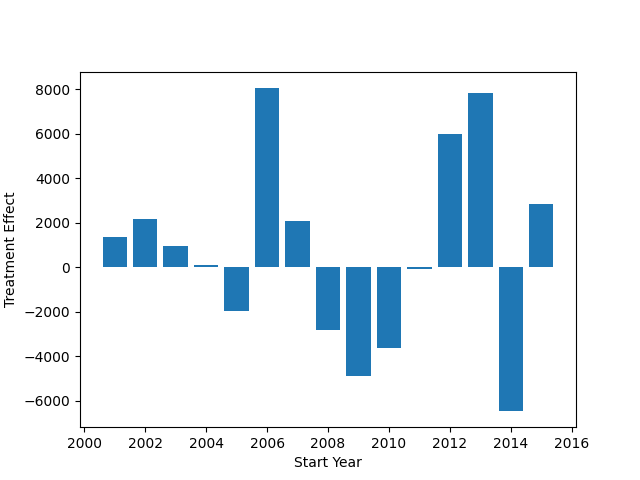
\includegraphics[width=13cm]{Treatment_effect_mob2.png}
    \caption{Dollar Difference between Treatment and Control group}
\end{figure}

\begin{figure}
    \centering
    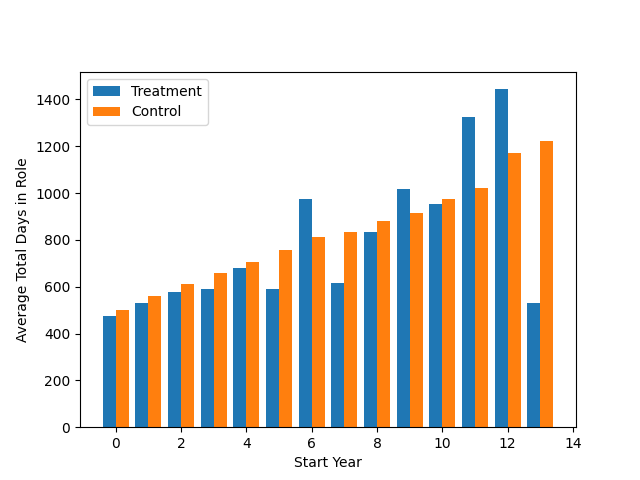
\includegraphics[width=13cm]{Time_in_role.png}
    \caption{Average time in role at Amazon and in Control}
\end{figure}

\begin{figure}[H]
\centering
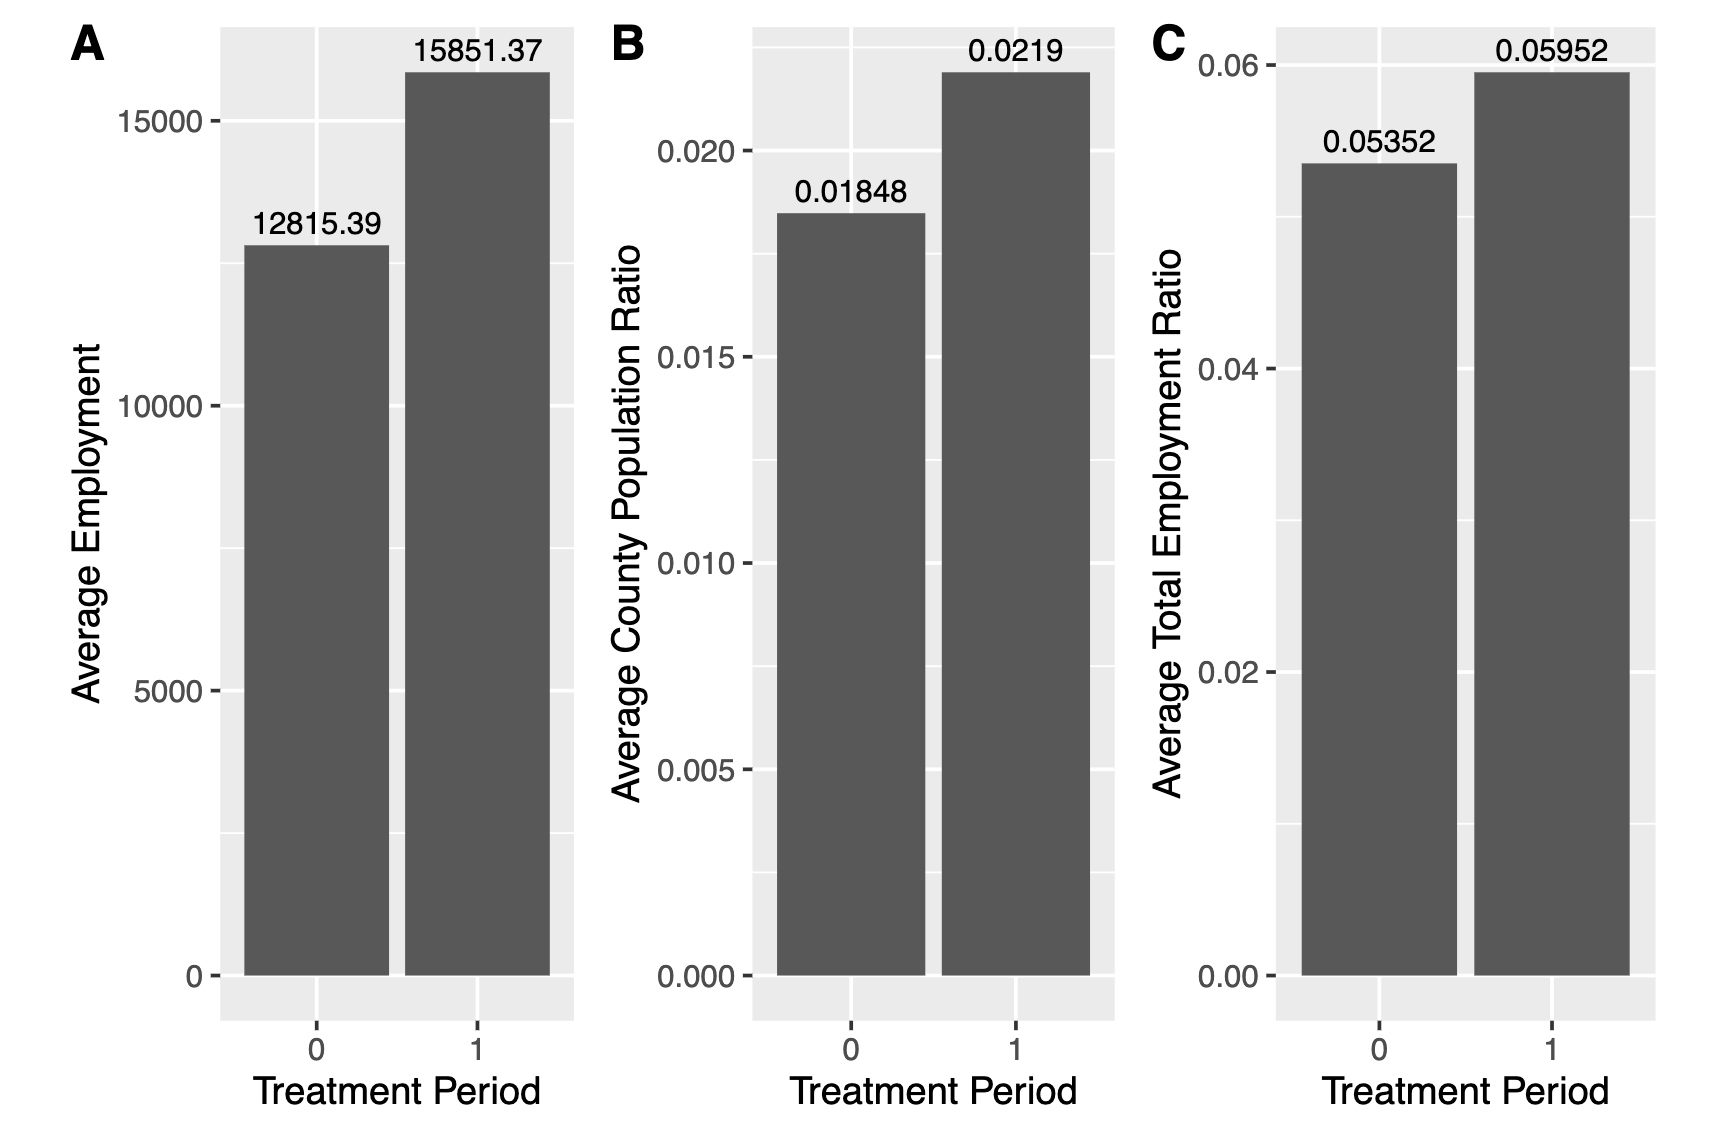
\includegraphics[width=15cm]{CONSTR.png}
\caption{Construction employment 2 years before and 2 years after Amazon Fulfillment Center openings}
\end{figure}

\begin{figure}[H]
\centering
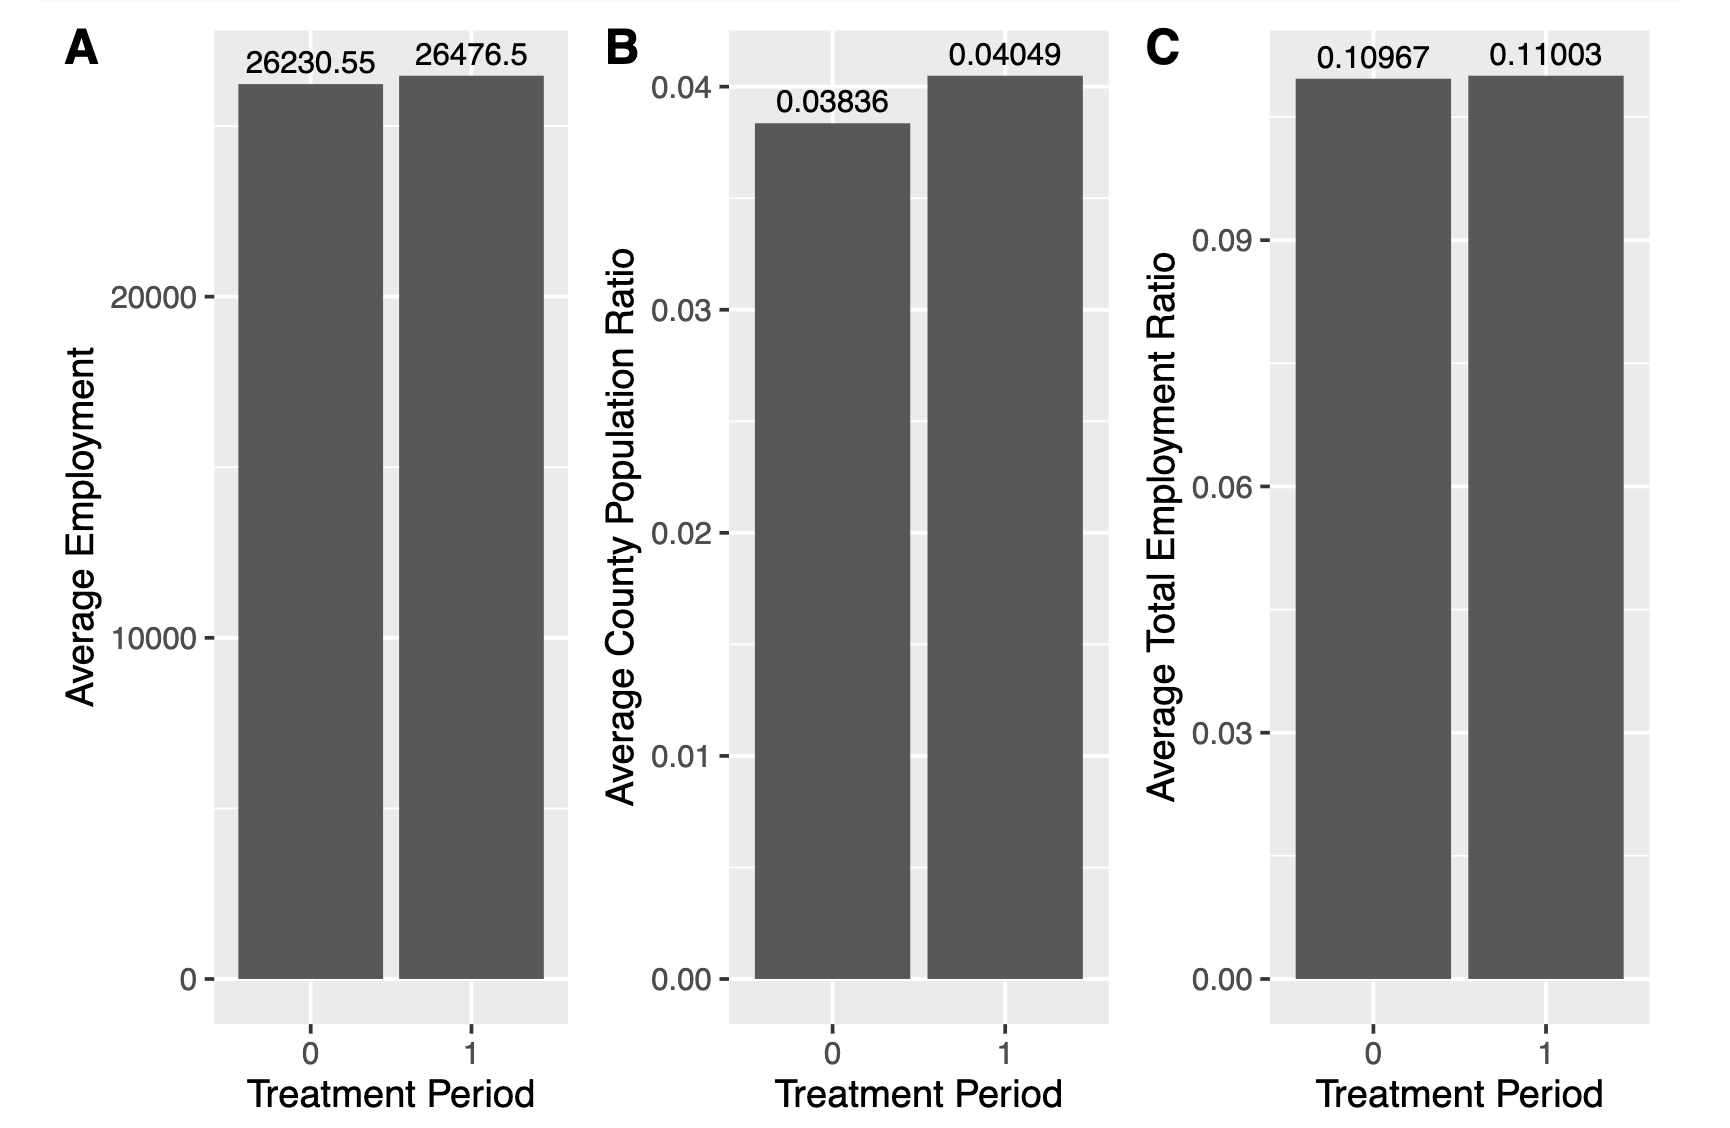
\includegraphics[width=15cm]{FOODMF.png}
\caption{Food Manufacturing employment 2 years before and 2 years after Amazon Fulfillment Center openings}
\end{figure}

\begin{figure}[H]
\centering
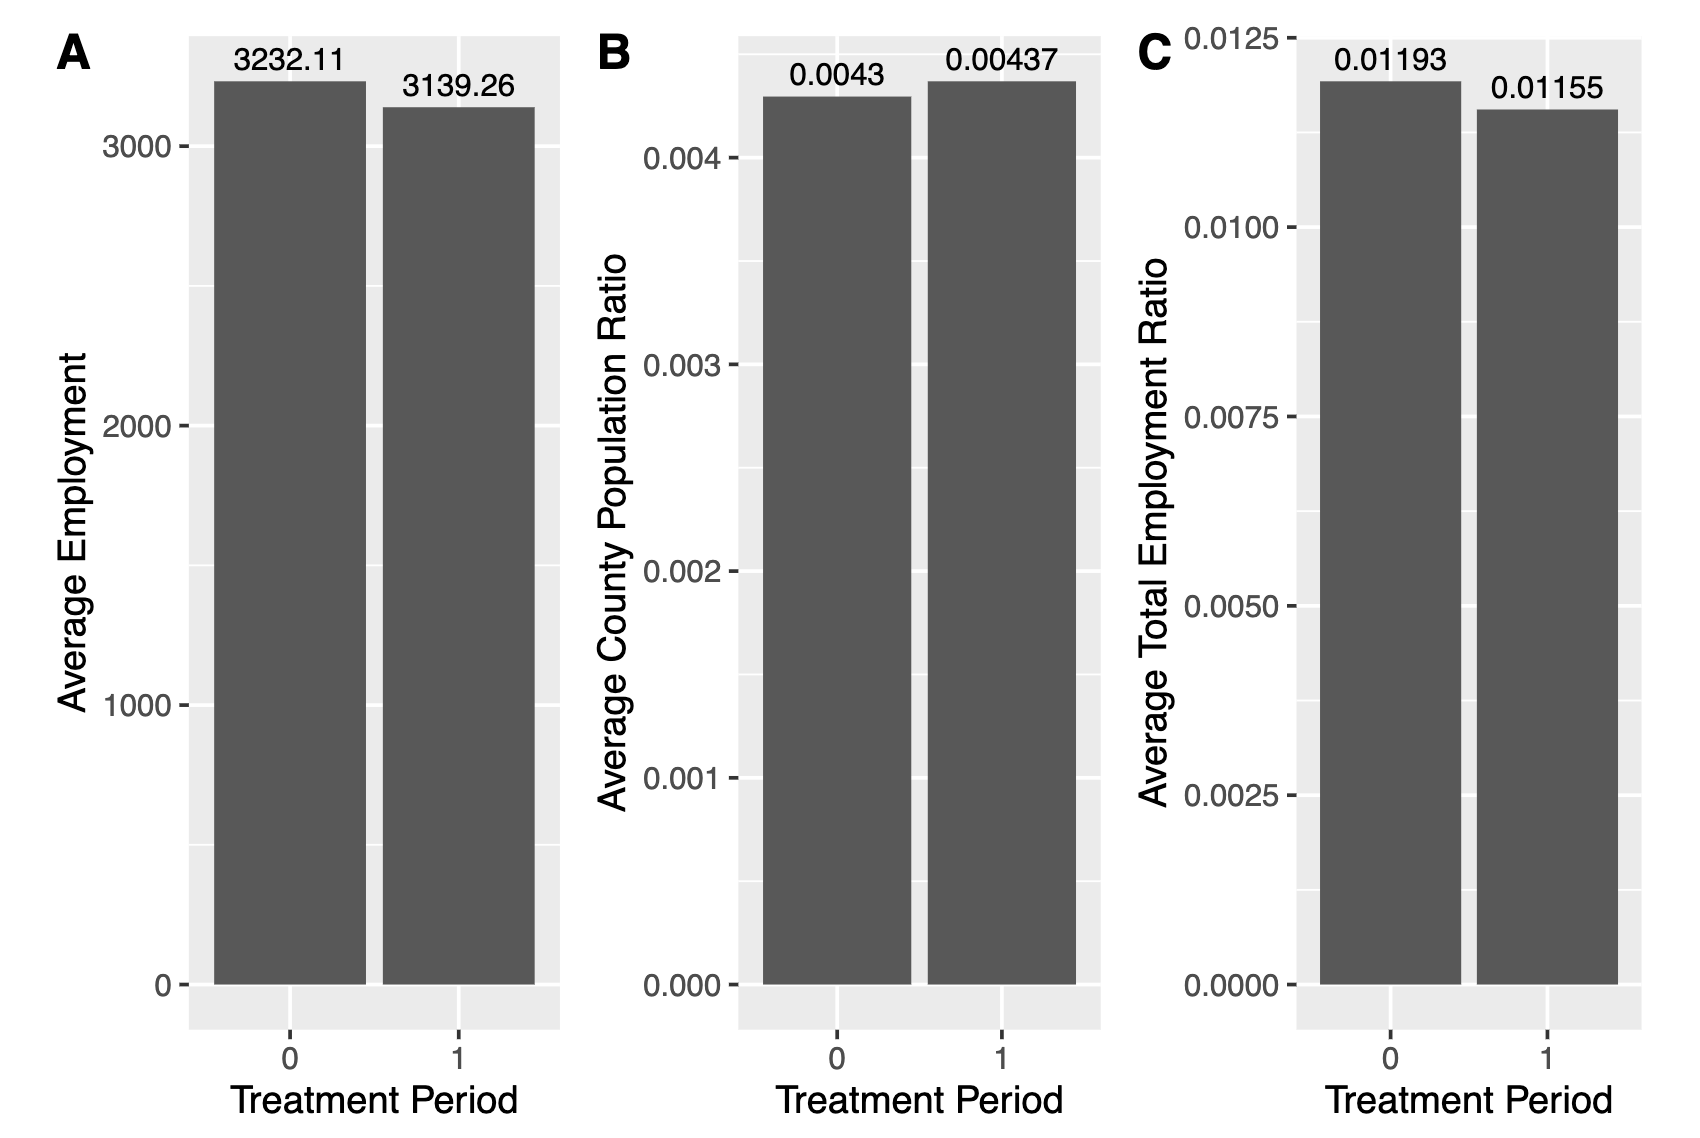
\includegraphics[width=15cm]{FABMETMF.png}
\caption{Fabricated Metals Manufacturing employment 2 years before and 2 years after Amazon Fulfillment Center openings}
\end{figure}

\begin{figure}[H]
\centering
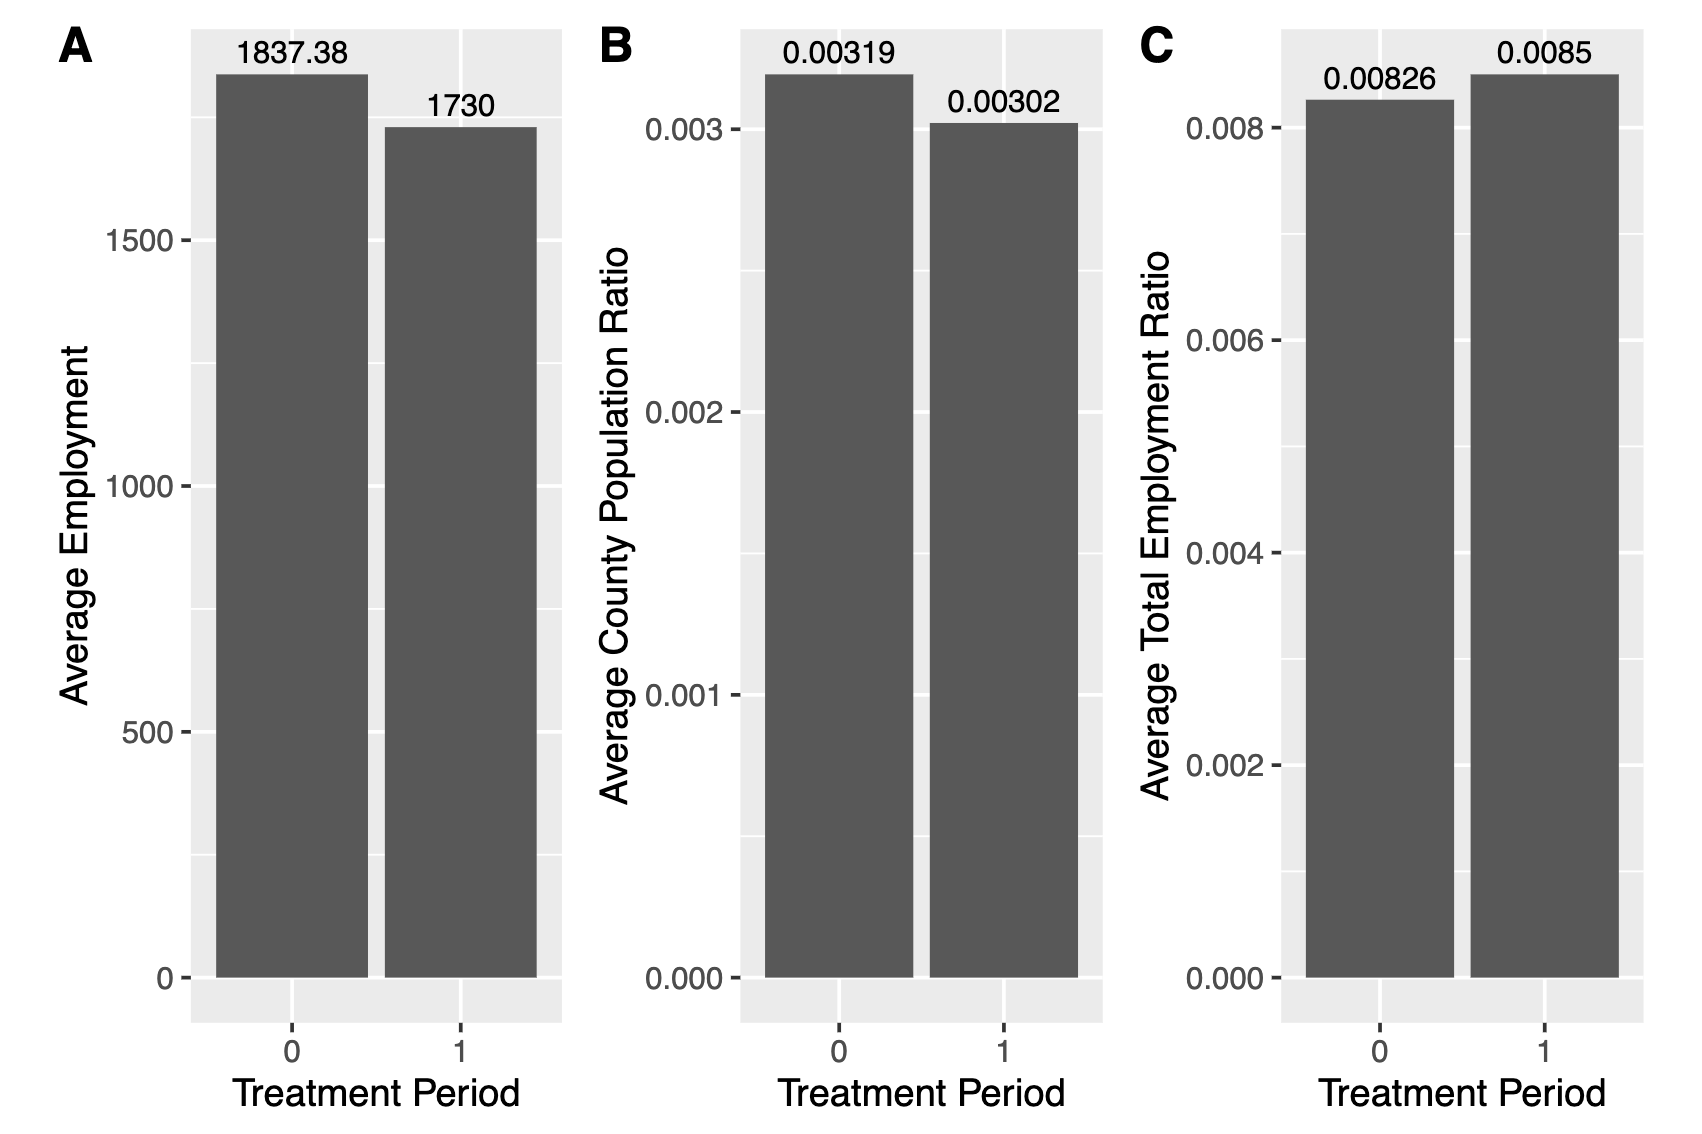
\includegraphics[width=15cm]{MACHMF.png}
\caption{Machinery Manufacturing employment 2 years before and 2 years after Amazon Fulfillment Center openings}
\end{figure}

\begin{figure}[H]
\centering
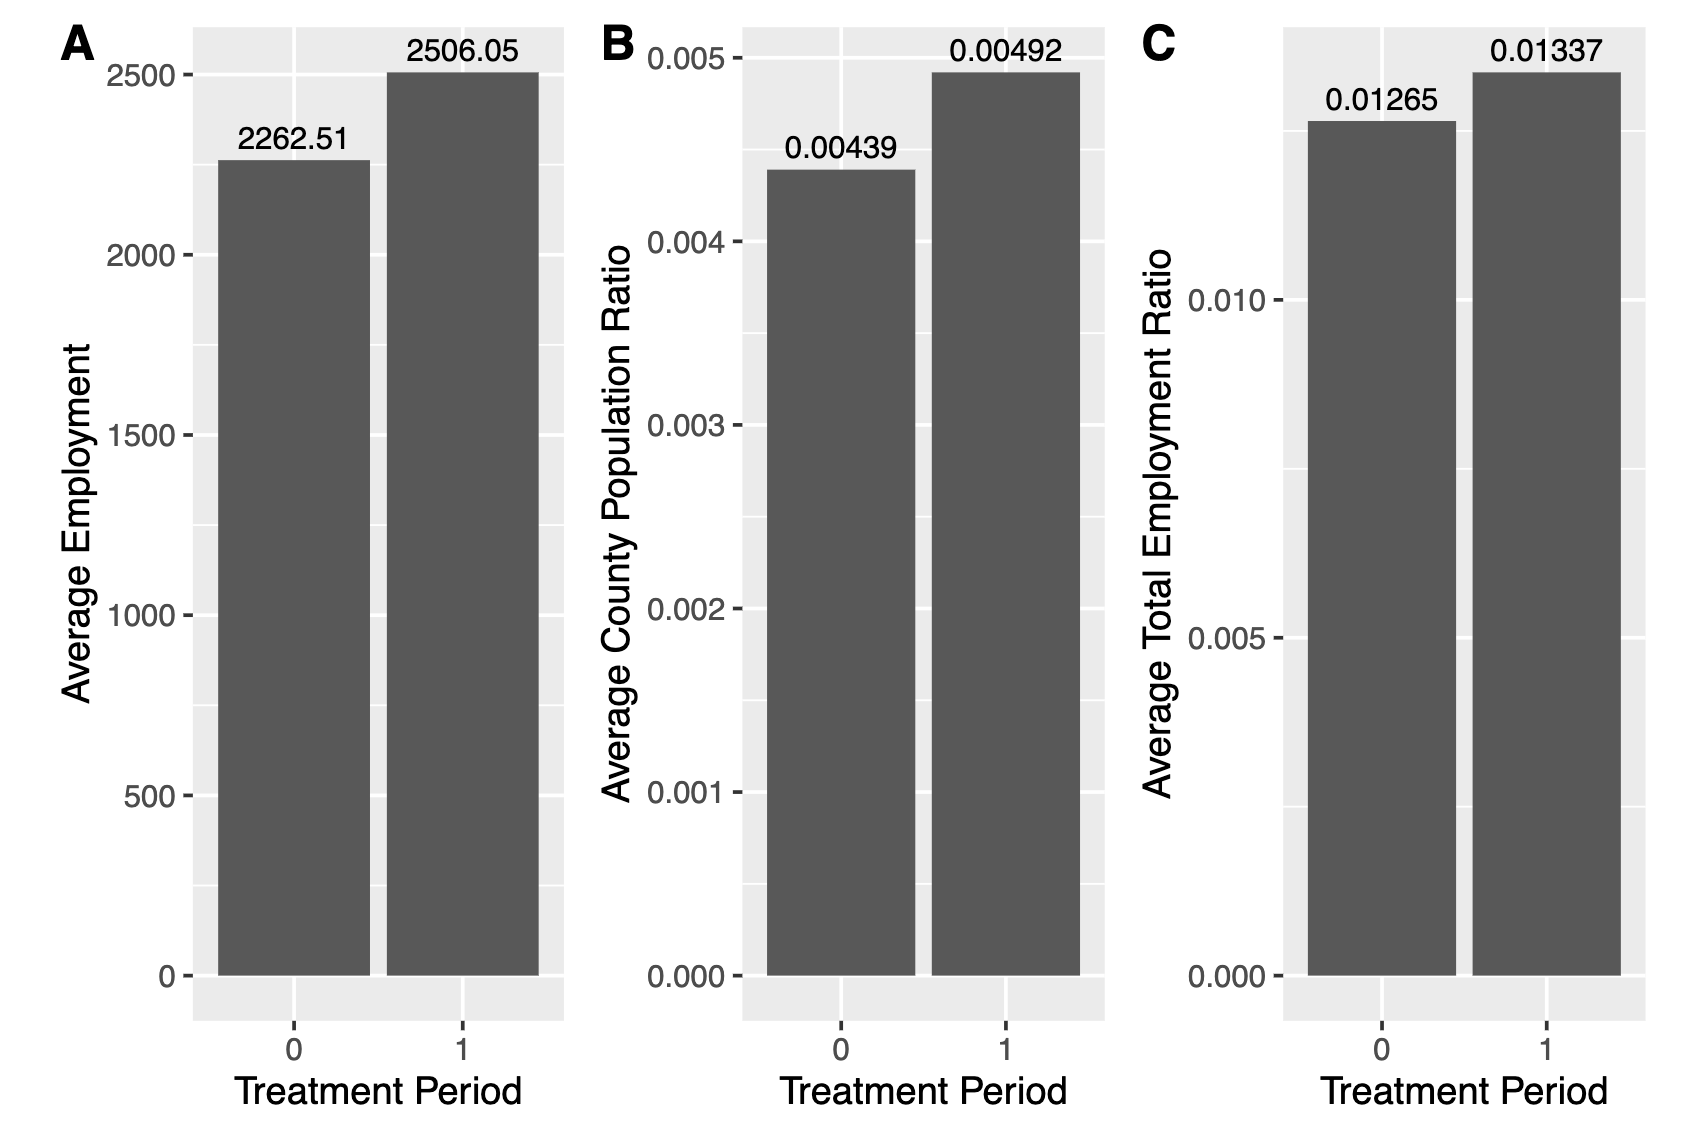
\includegraphics[width=15cm]{FRTRUCK.png}
\caption{Freight Trucking employment 2 years before and 2 years after Amazon Fulfillment Center openings}
\end{figure}

\begin{figure}[H]
\centering
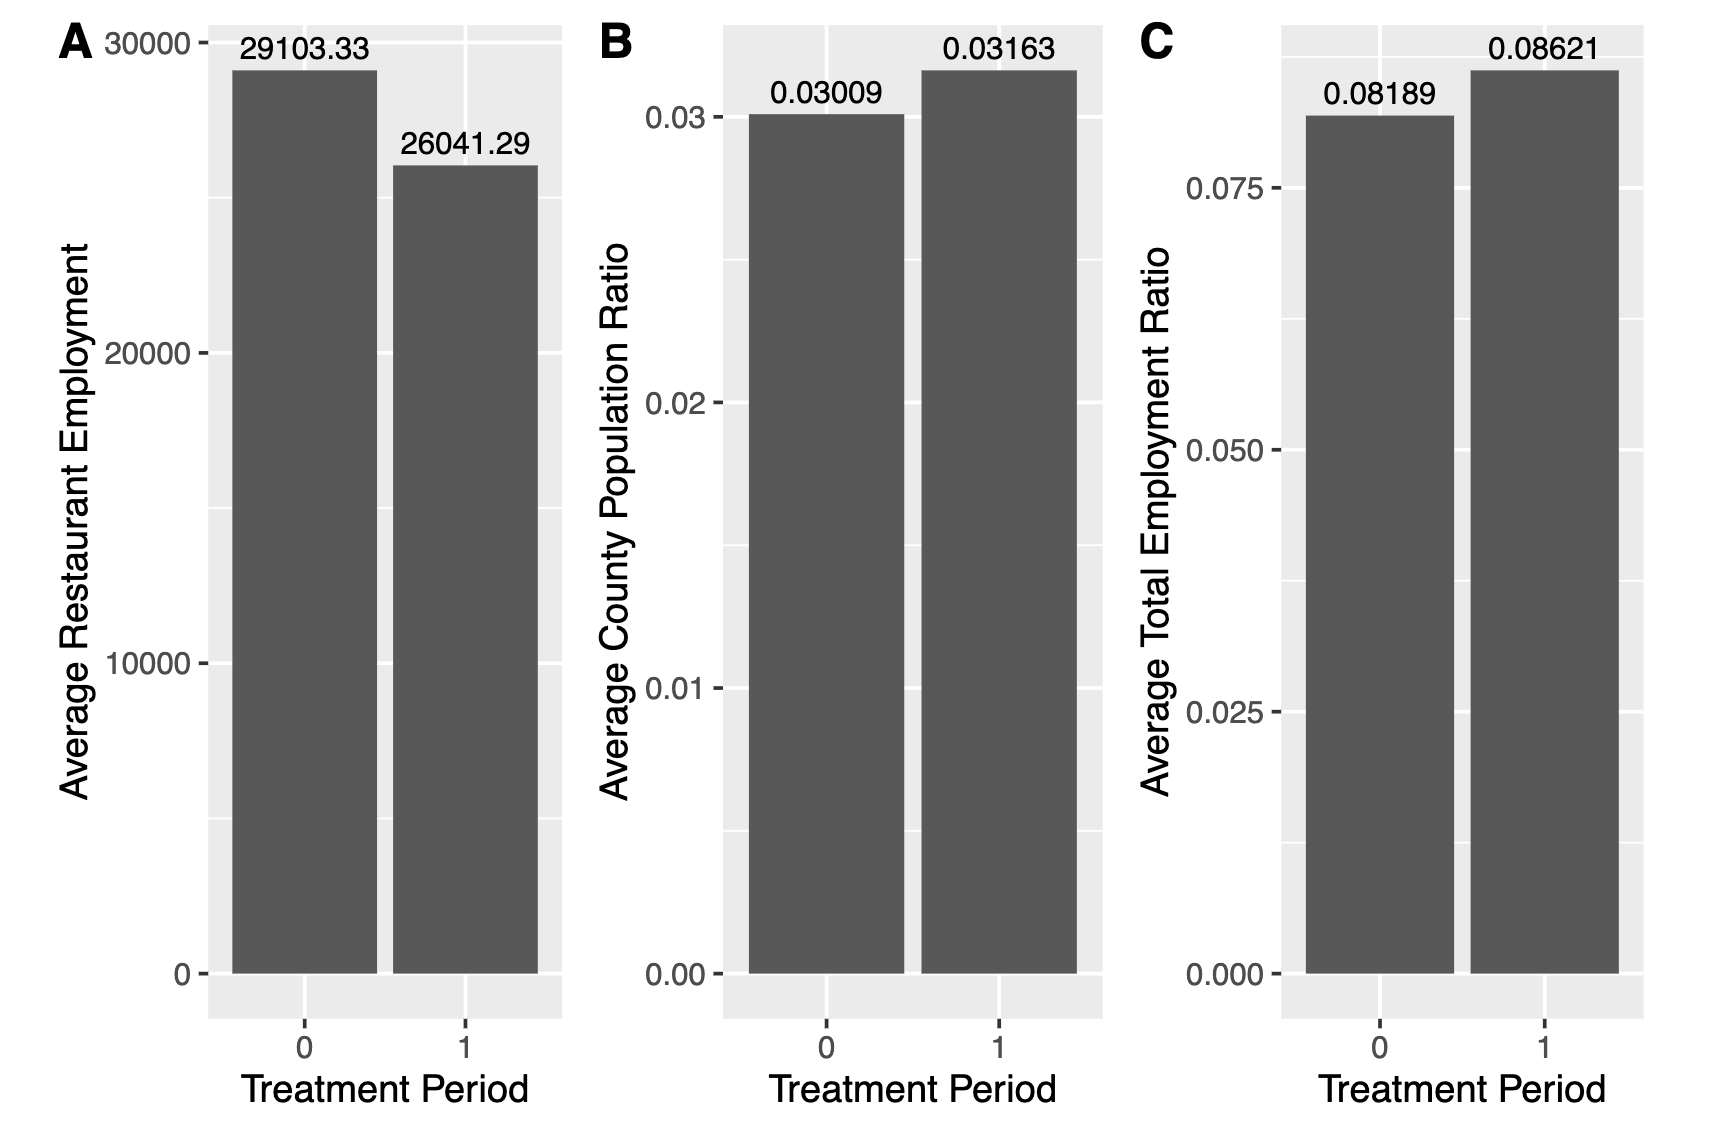
\includegraphics[width=15cm]{REST.png}
\caption{Restaurants and Other Eating Places employment 2 years before and 2 years after Amazon Fulfillment Center openings}
\end{figure}

\begin{figure}[H]
\centering
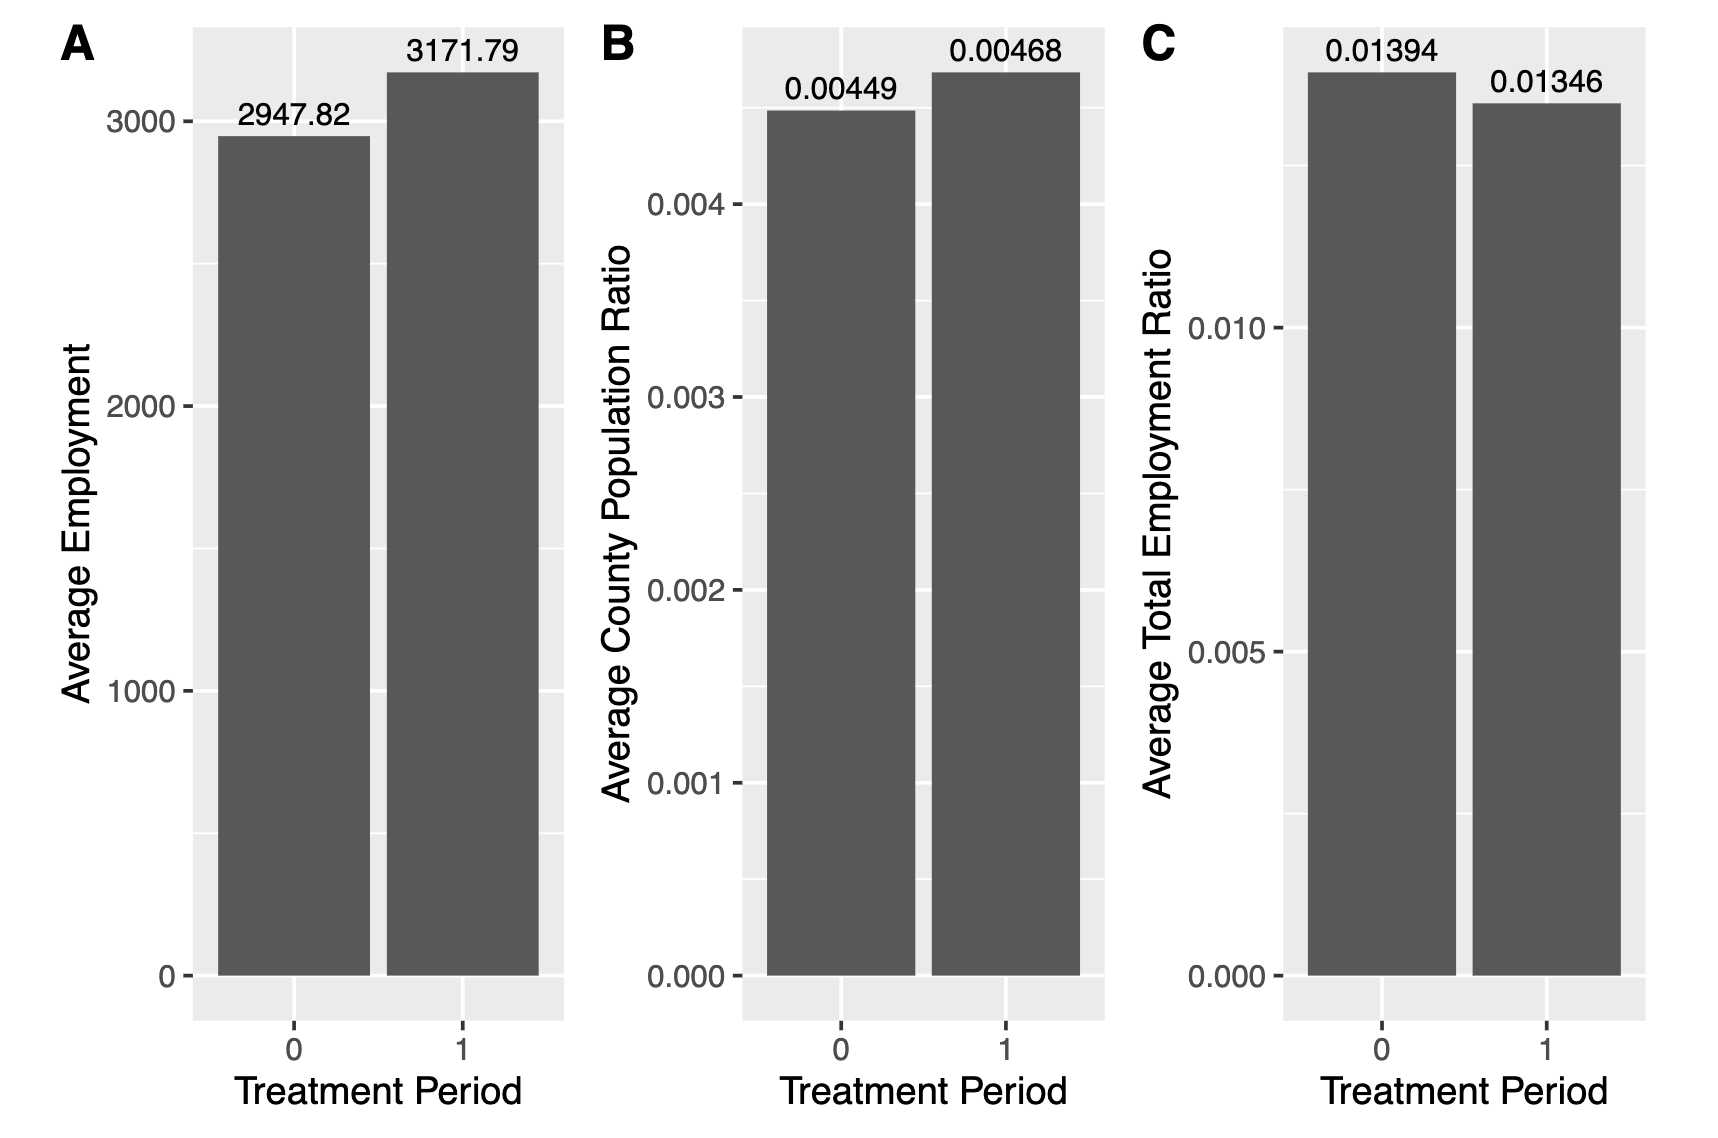
\includegraphics[width=15cm]{REPMT.png}
\caption{Repair and Maintenance employment 2 years before and 2 years after Amazon Fulfillment Center openings}
\end{figure}

\begin{figure}[H]
\centering
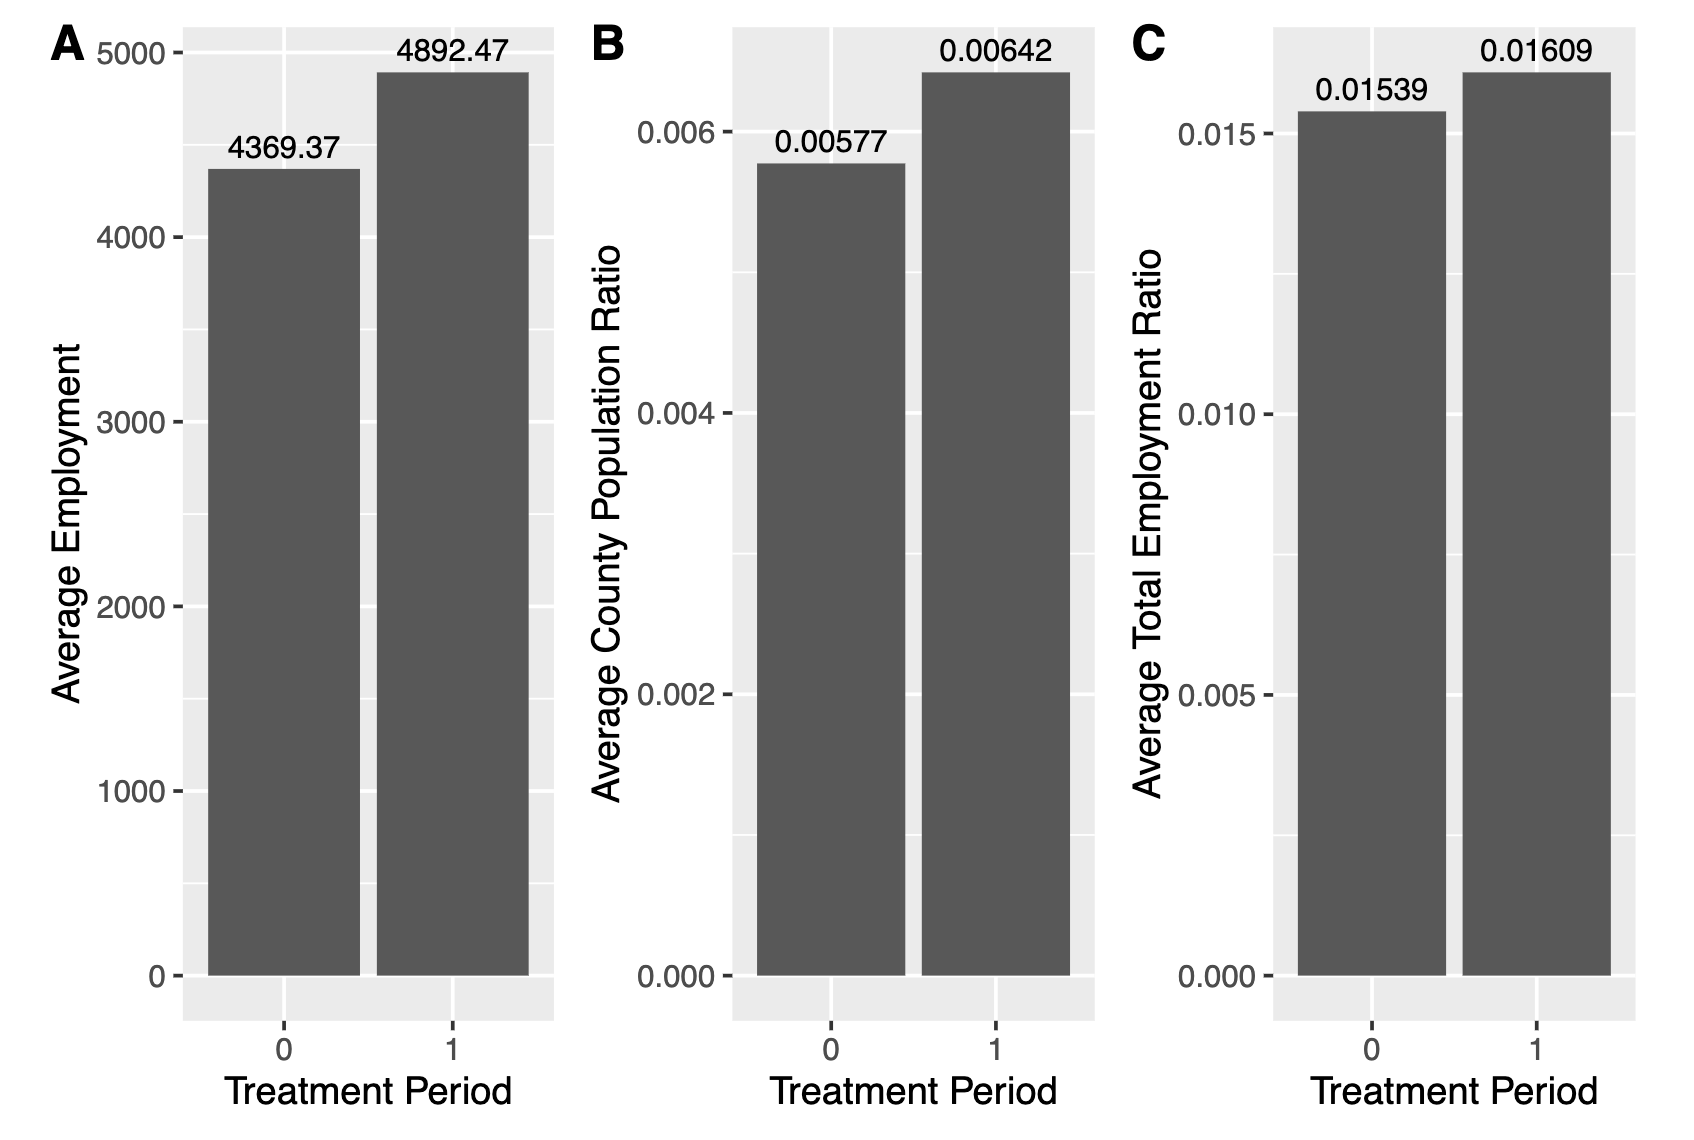
\includegraphics[width=15cm]{SERVBUILD.png}
\caption{Services to Buildings and Dwellings employment 2 years before and 2 years after Amazon Fulfillment Center openings}
\end{figure}

\begin{figure}[H]
\centering
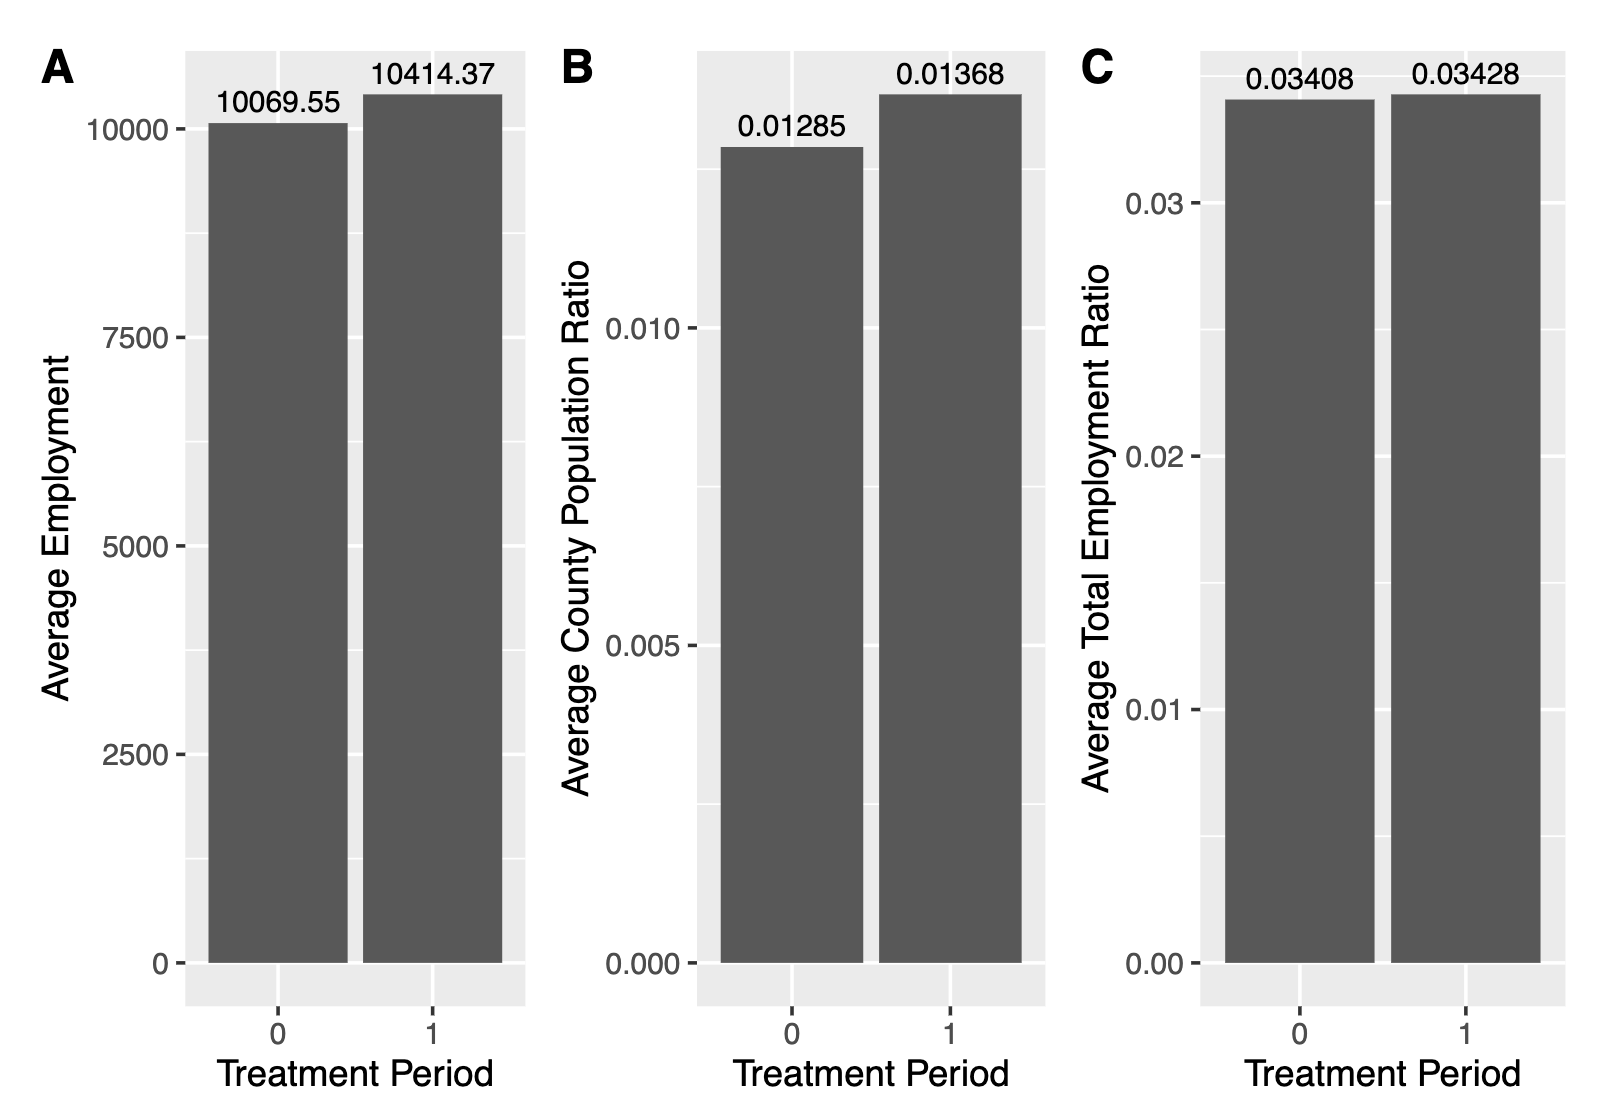
\includegraphics[width=15cm]{WHOLE.png}
\caption{Merchant Wholesalers (Durable Goods) employment 2 years before and 2 years after Amazon Fulfillment Center openings}
\end{figure}

\end{document}
1. Department of Labor, Occupational Safety and Health Administration, US DEPARTMENT OF LABOR FINDS AMAZON EXPOSED WORKERS TO UNSAFE CONDITIONS, ERGONOMIC HAZARDS AT THREE WAREHOUSES, 2022, Washington, DC

2. Department of Labor, Bureau of Labor Statistics, Warehousing and Storage,  NAICS Report 493, 1994-2023, Raw Data, Washington, DC

3. Timo has

4. Timo has

5. Timo has

6. Timo has


7. Fritsch, M., and Schindele, Y. (2011). The contribution of new businesses to regional employment-an empirical analysis. Econ. Geogr. 87, 153–180. doi: 10.1111/j.1944-8287.2011.01113

8. Becker, Gary S., and Nigel Tomes. “An Equilibrium Theory of
the Distribution of Income and Intergenerational Mobility.” Journal of Political Economy 87, no. 6 (1979): 1153–89. http://www.jstor.org/stable/1833328.

9. Chetty, Raj, Nathaniel Hendren, Patrick Kline,
Emmanuel Saez, and Nicholas Turner. 2014. ”Is the United States Still a Land of Opportunity? Recent Trends in Intergenerational Mobility.” American Economic Review, 104 (5): 141-47. DOI: 10.1257/aer.104.5.14

10. Reese, Ellen, Alexander Scott. 2019. "Warehouse Employment as a Driver of Inequality in the Inland Empire: The Experiences of Young Amazon Warehouse Workers." University of California at Berkeley. Othering & Belonging Institute.

11. De Lara, Juan. 2014. "Warehouse Work: Path to the Middle Class or Road to Economic Insecurity?" USC Program for Environmental and Regional Equity: 1-8.

12. OECD (2022), Supporting transitions and securing jobs: Social dialogue shaping a stronger recovery from the pandemic, https://www.oecd.org/coronavirus/policy-responses/supporting-transitions-and-securing-jobs-social-dialogue-shaping-a-stronger-recovery-from-the-pandemic-83b6b310/#boxsection-d1e37

13. Becker, Gary S. “Investment in Human Capital: A Theoretical Analysis.” Journal of Political Economy 70, no. 5 (1962): 9–49. http://www.jstor.org/stable/1829103. 

14. Babcock, L., Congdon, W.J., Katz, L.F. et al. 2012. "Notes on behavioral economics and labor market policy." IZA J Labor Policy 1, 2 (2012). https://doi.org/10.1186/2193-9004-1-2

15. Davis, Otto A., and Andrew B. Whinston. “The Economics of Urban Renewal.” Law and Contemporary Problems 26, no. 1 (1961): 105–17. https://doi.org/10.2307/1190601.

16. “Viguie, V.; Hallegatte, S.. 2014. Urban Infrastructure Investment and Rent-Capture Potentials. Policy Research Working Paper;No. 7067. © World Bank Group, Washington, DC. http://hdl.handle.net/10986/20513